\documentclass[main.tex]{subfiles}
\begin{document}
\chapter{Tools for calculating scattering amplitudes} \label{sec:tools}
In this chapter, we focus on various aspects of the computation of loop scattering amplitudes for high-multiplicity processes. It is important to note that there is currently no one-size-fits-all approach that would allow us to compute all the desired amplitudes at a press of a button. In practice, we use a collection of methods that are most appropriate for the task at hand. For processes at the limit of current capabilities, these tools need to be further improved or replaced with novel ideas. To this end, much work has been done by the theory community in recent years. Unfortunately, due to the overwhelming algebraic and analytic complexity, many calculations still present challenges beyond the reach of current technology. 
\begin{figure}[t]
\begin{tikzpicture}
	\node (feynman) [greenrec] {Feynman diagrams};
	\node (colour)  [redrec,right of=feynman,xshift=4cm] {Colour decomposition};
	\node (topos)   [redrec,right of=colour,xshift=4cm] {Helicity amplitudes};
	\node (reduction) [bluerec,below of=topos,yshift=-2cm] {\parbox{0.3\textwidth}{\centering Integrand reduction onto \\ maximal topologies}};
	\node (IBPs)    [bluerec,left of=reduction,xshift=-4cm] {IBP reduction};
	\node (spfns)   [bluerec,left of=IBPs, xshift=-4cm] {\parbox{0.3\textwidth}{\centering Expansion of MIs onto \\ a special function basis}};
	\node (sub)     [bluerec,below of=spfns,yshift=-2cm] {Pole subtraction};
	\node (finrem)  [bluerec,right of=sub,xshift=4cm] {Finite remainder};
	\node (rec)  [bluerec,right of=finrem,xshift=4cm] {Reconstruction};
	\node (qgraf) [below of=feynman, opacity=0.7] {\textcolor{green}{\Large QGRAF}};
	\node (mma) [below right of=colour, xshift=1.5cm, yshift=-0.3cm, opacity=0.7] {\textcolor{red}{\Large Mathematica/FORM}};
	\node (ff) [below of=IBPs, yshift=-0.5cm,opacity=0.7] {\textcolor{blue}{\Large finite fields}};
		
	\draw[->] (feynman.east) -- (colour.west);
	\draw[->] (colour.east) -- (topos.west);
	\draw[->] (topos.south) -- (reduction.north) node[midway,right] {$d=4-2\epsilon$};
	\draw[->] (reduction.west) -- (IBPs.east);
	\draw[->] (IBPs.west) -- (spfns.east);
	\draw[->] (spfns.south) -- (sub.north);
	\draw[->] (sub.east) -- (finrem.west) node[midway,above] {$\epsilon \rightarrow 0$};
	\draw[->] (finrem.east) -- (rec.west);
\end{tikzpicture}
\caption{A schematic overview of the workflow we adopt to compute scattering amplitudes.}
\label{fig:outline}
\end{figure}
The goal of this chapter is to provide an overview of the methods we adopt in amplitude computations, as well as the problems that invariably follow. The procedure involves several highly non-trivial steps. To help the reader retain the `big picture' of the workflow, we present its schematic outline in Fig.~\ref{fig:outline}. Each step is discussed in more detail below. 
\section{Feynman diagrams}
The starting point of our amplitude computation for a given process is the generation of all Feynman diagrams contributing to this process at the desired loop order. Feynman diagrams provide a pictorial representation of the ways in which the interaction can occur. At the same time, the corresponding Feynman integrals can be easily recovered using Feynman rules, which can be derived from the Lagrangian of the theory under consideration. As such, these diagrams are an indispensable tool of any perturbative calculation. In practice, it can be observed that usually their number grows faster than exponentially as we increase the loop order or multiplicity (see Table~\ref{tab:ndiags} for an example). To handle the combinatorial complexity, we generate the relevant Feynman diagrams using $\texttt{QGRAF}$~\cite{Nogueira:1991ex}. This programme has the advantage of granting the user a large degree of control over the output. For example, one can constrain it to generate diagrams without self-energy insertions or with a specified total power of the coupling constant.
\begin{table}[b]
	\begin{center}
		\begin{tabular}{r|c|c|c|c|c|c|c|c}
			  $n$ & 1 & 2 & 3 & 4 & 5 & 6 & 7 & 8 \\
			\hline
			$n$ gluons   & -- & -- & 1 & 4 & 25 & 220 & 2485 & 34300 \\
			$q\bar{q} + n$ gluons & 1 & 3 & 16 & 123 & 1240 & 15495 & 231280 & 4016775 \\
		\end{tabular}
	\end{center}
 \caption{Number of tree-level diagrams contributing to selected processes with $n$ gluons.}
 \label{tab:ndiags}
\end{table}
\section{Colour decomposition} \label{sec:colourdec}
Having generated the Feynman diagrams, we substitute the Feynman rules for the propagators and vertices using \texttt{Mathematica}. At this point, our QCD amplitude contains both colour and kinematic information. The idea of colour ordering is to reorganise the amplitude such that these two components separate: a purely kinematic part is multiplied by the corresponding colour factor. In other words, we perform the decomposition of the full amplitude in colour space, according to a chosen colour basis. Roughly speaking:
\begin{equation}
    \ampl{n}{} = \sum_i \text{(colour)}_i \times A_{n\,i} \,, 
\end{equation}
where $A_{n\,i}$ are the colour-ordered amplitudes (also known as colour-stripped or partial amplitudes). The motivation behind this decomposition is that the colour-ordered amplitudes turn out to be significantly simpler to calculate.

The choice of the colour basis is not unique. We adopt the decomposition according to traces of the $SU(N_c)$ generators in the fundamental representation. As an example, let us look at 4-gluon scattering at tree-level. The $s$-channel diagram is:
\begin{equation} \label{eq:3grule}
\feynmandiagram [baseline = (i.base), horizontal = i to j] {
    a1 [particle={$A^{a_2}_{\mu_2}(p_2)$}] -- [gluon] i;
    a2 [particle={$A^{a_1}_{\mu_1}(p_1)$}] -- [gluon] i;
    i -- [gluon] j;
    a3 [particle={$A^{a_4}_{\mu_4}(p_4)$}] -- [gluon] j;
    a4 [particle={$A^{a_3}_{\mu_3}(p_3)$}] -- [gluon] j;
    };
    \xrightarrow{\text{colour}}
    f^{a_1a_2b}f^{ba_3a_4} \,.
\end{equation}
The colour factor of this diagram can be expressed in terms of the generators using Eqs.~\ref{eq:fierzcolour} and \ref{eq:fabc}:
\begin{align}
    f^{a_1a_2b}f^{ba_3a_4} = -\frac{1}{T_F} &\big(\tr[T^{a_1} T^{a_2} T^{a_3} T^{a_4}] - \tr[T^{a_1} T^{a_2} T^{a_4} T^{a_3}] \nonumber \\
    & - \tr[T^{a_1} T^{a_3} T^{a_4} T^{a_2}] + \tr[T^{a_1} T^{a_4} T^{a_3} T^{a_3}]\big) \,.
\end{align}
The colour factors of the $t$- and $u$-channels can be expressed in a similar way. Combining the contributions from the three channels and using the cyclicity of the trace, we can organise the 4-gluon amplitude at tree-level as follows:
\begin{equation}
    \ampl{4}{(0)} =  g_s^2 \left( \tr[T^{a_1} T^{a_2} T^{a_3} T^{a_4}]\,A_{4}^{(0)}[1234] + \text{permutations of } (234) \right) \,,
\end{equation}
where we have factored out $g_s^2/(4\pi) \equiv \alpha_s$ for convenience. In the general case, this formula reads:
\begin{equation} \label{eq:colour-decomposition}
    \ampl{n}{(0)} = g_s^{n-2} \sum_{\sigma \in S_{n-1}} \tr\left[T^{a_1} T^{\sigma(a_2} \ldots T^{a_n)}\right] A_n^{(0)} \left[1\,\sigma(2\ldots n)\right] \, ,
\end{equation}
where the sum is over the set of all \textit{non-cyclic} permutations of $n-1$ particles. Similar colour decompositions can be derived for amplitudes involving quarks, as well as beyond tree-level~\cite{Dixon:1996wi}. At loop level, in addition to single-trace structures the colour basis contains products of traces.

The colour-ordered amplitudes $A_n$ are calculated by adding up the kinematic parts of all Feynman diagrams contributing to a given colour factor. They are gauge invariant and satisfy a number of important identities~\cite{Mangano:1990by, Kleiss:1989616, Bern:2008qj}:
\begin{align}
    A_n[123\ldots n] &= A_n[23\ldots n\,1]\,, && \text{cyclicity}, \\
    A_n[123\ldots n] &= (-1)^n A_n[n \ldots 321] \,, && \text{reflection}, \\
    A_n[123 \ldots n] &+ \mathrlap{A_n[213 \ldots n] +  A_n[231 \ldots n] +  \ldots + A_n[23 \ldots 1\,n] = 0 \,,} && \nonumber \\ 
    & && U(1) \text{ decoupling}, \\
    A_n[1, {\alpha}, n, {\beta}] &= (-1)^{|\beta|} \sum_{\mathclap{\sigma \in OP(\{\alpha\} \cup \{\beta^T\})}} A_n[1, \sigma, n] \,, && \text{Kleiss-Kuiff relations}.
\end{align}
In the last line, the sum runs over permutations in the joint set $\{\alpha\} \cup \{\beta^T\}$ such that the order within the individual sets is preserved, and $\{\beta^T\}$ is the reversal of the set $\{\beta\}$. Crucially, these properties allow us to reduce the number of independent amplitudes that need to be computed. In fact, for $n$-gluon scattering, this number is just $(n-2)!$\,.

\section{Helicity amplitudes}
After colour decomposition, our colour-ordered amplitude contains purely kinematic information. The kinematic part of the Feynman rules for external states carries information about the spins and polarisations of particles: for massless spin\=/1/2 fermions, we use $\pm$ helicity states to differentiate between the two solutions to the Dirac equation, while for massless spin\=/1 bosons, they denote the two polarisation vectors. From the experimental perspective, we are rarely interested in differentiating between the spin states of individual particles. Usually, a beam of particles with random spins undergoes scattering and we look at the total number of products outgoing in a certain direction. Thus, to calculate the corresponding cross section, we should average over the initial spin states and sum over the final ones. This can be achieved in two different ways: 
\begin{enumerate}
    \item Perform the amplitude calculation without specifying the helicity states, i.e. square the amplitude, then do the spin sums that appear at the level of $|\ampl{}{}|^2$ using completeness relations of Eqs.~\ref{eq:completeness:fermions} and \ref{eq:completeness:bosons}.
    \item Specify the helicity states of external particles, compute each \textbf{helicity amplitude} separately, square them and sum over all relevant helicity configurations.
\end{enumerate}
In our approach, we will adopt the latter method. We denote an $L$-loop helicity amplitude as:
\begin{equation} \label{eq:helampdef}
    \ampl{n}{(L),\,\{h\}} \equiv \ampl{n}{(L)}(1^{h_1}2^{h_2} \ldots n^{h_n})\,,
\end{equation}
where the superscript $\{h\}$ is understood as the set of helicities $h_i$ of the $n$ particles, but will be usually omitted since we will exclusively compute helicity amplitudes. The full, spin-summed amplitude can then be recovered through:
\begin{equation}
    \ampl{n}{(L)} = \sum_{\mathclap{\substack{\text{helicity} \\ \text{configurations}}}} \ampl{n}{(L),\,\{h\}} \,.
\end{equation}
At the cross section level, we get:
\begin{equation}
    \left|\ampl{n}{(L)}\right|^2 = \sum_{\mathclap{\substack{\text{helicity} \\ \text{configurations}}}} \left|\ampl{n}{(L),\,\{h\}} \right|^2 \,.
\end{equation}
It is important to note that this sum includes only the squares of individual helicity amplitudes --- there are no interferences between different helicity configurations.

There are several strong advantages to this approach. Firstly, we can see that the number of terms that need to be processed is significantly smaller than in method~(1). Consider the expansion of an amplitude in the coupling constant $\alpha$ up to two loops:
\begin{equation}
    \ampl{}{} = \ampl{}{(0)} + \alpha \ampl{}{(1)} + \alpha^2 \ampl{}{(2)} + \order{\alpha^3} \,.
\end{equation}
Then, at the level of the cross section, we have the following contributions:
\begin{equation}
    |\ampl{}{}|^2 = |\ampl{}{(0)}|^2 \,+\,\alpha\,2\,\mathrm{Re}\left(\ampl{}{(0)\ast}\ampl{}{(1)}\right) \,+\, \alpha^2 \left(2\,\mathrm{Re} \left(\ampl{}{(0)\ast}\ampl{}{(2)}\right) + |\ampl{}{(1)}|^2 \right) \,+\, \order{\alpha^3}\,.
\end{equation}
Let us also schematically write each $L$-loop amplitude as a sum of $m_L$ Feynman diagrams: $\ampl{}{(L)} = d^{(L)}_1 + d^{(L)}_2 + \ldots + d^{(L)}_{m_L}$. Then, at tree level:
\begin{equation}
    \left|\ampl{n}{(0)}\right|^2 = \sum_{\mathclap{\substack{\text{hel.} \\ \text{confs.}}}} \left|\ampl{n}{(0),\,\{h\}} \right|^2 = \sum_{\mathclap{\substack{\text{hel.} \\ \text{confs.}}}} \left|d^{(0)\,,\{h\}}_1 + d^{(0)\,,\{h\}}_2 + \ldots + d^{(0)\,,\{h\}}_{m_0} \right|^2 \,.
\end{equation}
Each term in this sum has all helicities fixed and there are no spin sums to be performed (when evaluated at a chosen phase-space point, it is just a complex number). Thus, the number of terms we need to process at LO is $m_0 n_h$, where $n_h$ is the number of independent helicity configurations. On the other hand, according to method (1), we have:
\begin{equation}
    \left|\ampl{n}{(0)}\right|^2 = \left(d^{(0)}_1 + d^{(0)}_2 + \ldots + d^{(0)}_{m_0} \right) \left(d^{(0)\ast}_1 + d^{(0)\ast}_2 + \ldots + d^{(0)\ast}_{m_0} \right)\,,
\end{equation}
which means we need to interfere the diagrams with each other and perform the spin sums. Thus, there are $m_0^2$ terms to be processed. The scaling for higher loop orders is listed in Table~\ref{tab:nterms}. For small $L$, the advantage of using helicity amplitudes might be minimal (or in fact, it might be detrimental to do so). For $L\geq2$, however, the advantage becomes apparent, especially that due to the symmetries of colour-ordered amplitudes, $n_h$ is usually much smaller than $2^n$. Moreover, it turns out that not all helicity amplitudes are equally challenging to compute, as we will see in the next section. In fact, a host of them vanish altogether (at least at tree-level). We remark that guided by experience, it is possible to choose the reference vectors of external polarisations such that the computation of the non-zero amplitudes becomes easier. Helicity amplitudes can also provide us with more information about the scattering process, for example when working with polarised cross sections. In Chapters~\ref{sec:Wyj} and~\ref{sec:QEDpaper}, we will see how we can use them to attach the decay current of the $W$ boson and an off-shell photon, respectively, to an amplitude with an off-shell leg in order to obtain an amplitude for a fully on-shell process at a higher multiplicity.

When dealing with helicity amplitudes, it is conventional to introduce nomenclature encoding the number of positive/negative helicity particles involved in the process. Consider $2\rightarrow (n-2)$ gluon scattering where the outgoing momenta all have opposite helicities to the incoming ones: $1^-2^- \rightarrow 3^+ \ldots n^+$. We call such a configuration `helicity violating'. We can cross particles 1 and 2 to the final state, which changes their helicities: $0\rightarrow 1^+2^+ \ldots n^+$. This corresponds to the `all-plus' amplitude $A_n(1^+2^+ \ldots n^+)$ with all momenta outgoing. In the next section, we will show that for gluon scattering at tree-level, this amplitude vanishes for all $n$. If we flip one helicity in the final state: $1^-2^- \rightarrow 3^- \ldots n^+$, this corresponds to $A_n(1^+2^+3^-4^+ \ldots n^+)$, which also turns out to vanish at tree-level. The first non-zero configuration is $1^-2^- \rightarrow 3^-4^- \ldots n^+$, which corresponds to: $A_n(1^+2^+3^-4^-5^+ \ldots n^+)$. For this reason, amplitudes with exactly two negative helicity particles are called \textbf{maximally helicity violating} (MHV). Similarly, amplitudes with exactly two positive helicities are known as anti-MHV. Furthermore, configurations with $2+k$ negative/positive helicities are referred to as $\text{N}^k\text{MHV}/\text{anti-N}^k\text{MHV}$. Tree-level MHV amplitudes are remarkably simple, as we will demonstrate in the next section. 
\begin{table}[t]
	\begin{center}
		\begin{tabular}{c|c|c|c}
			  \# terms & $L=0$ & $L=1$ & $L=2$ \\
			\hline
			Method (1) & $m_0^2$ & $m_0^2 + m_0 m_1$ & $m_0^2 + m_0 m_1 + m_1^2 + m_0 m_2$ \\
			Method (2) & $m_0 n_h$ & $(m_0+m_1)n_h$ & $(m_0+m_1+m_2)n_h$ \\
		\end{tabular}
	\end{center}
 \caption{Number of terms to be processed in the computation of the squared amplitude $\left|\ampl{}{}\right|^2$ \textit{up to and including} a given loop order, assuming there are $m_L$ diagrams at $L$ loops. The meaning of methods (1) and (2) is explained above Eq.~\ref{eq:helampdef}.}
 \label{tab:nterms}
\end{table}
\section{Spinor helicity formalism} \label{sec:spinhelform}
In Section~\ref{sec:QFTintro}, we saw that for massless particles, the Dirac spinor splits into two Weyl spinors that do not mix and are associated with the helicity of the particle. Therefore, we might be tempted to think that helicity amplitudes are better described using a notation specific to the two-component Weyl spinors, which are acted on by the familiar Pauli matrices. Indeed, the powerful spinor-helicity formalism provides a neat way to express helicity amplitudes based on these considerations\footnote{In case the notation that follows appears daunting, we refer the reader to Ref.~\cite{ElvangHuang} for an in-depth discussion of the topic and useful exercises.}.

As a first step, let us see how we can move from working with the four-component objects to two-component ones. We can write a `slashed' momentum $\slashed{p}$ as:
\begin{equation} \label{eq:pslashed1}
    \slashed{p} = p_\mu \gamma^\mu = p_\mu
    \begin{pmatrix}
    0 & (\sigma^\mu)_{a\dot{b}} \\
    (\bar{\sigma}^\mu)^{\dot{a}b} & 0
    \end{pmatrix}
    \equiv
    \begin{pmatrix}
    0 & p_{a\dot{b}} \\
    p^{\dot{a}b} & 0 
    \end{pmatrix} \,,
\end{equation}
with both dotted and un-dotted indices running over $\{1,2\}$ and $(\sigma^\mu)_{a\dot{b}} \equiv (1, \, \sigma^i)$, $(\bar{\sigma}^\mu)^{\dot{a}b} \equiv (1, \, -\sigma^i)$, where $\sigma^i$ are the three Pauli matrices. The momentum bispinors $p^{\dot{a}b}$ and $p_{a\dot{b}}$ can be thought of as $(2 \times 2)$ matrices and it is easy to show that:
\begin{equation}
    \det p_{a\dot{b}} = \det p^{\dot{a}b} = m^2\,.
\end{equation}
For massless particles, this determinant vanishes and the matrix can be expressed as an outer product of two vectors\footnote{The determinant of a matrix is 0 only if its column/row vectors are linearly dependent, which for a $(2 \times 2)$ matrix implies that its rank is 1. A rank-1, $(n \times m)$ matrix can always be expressed as the outer product of two nonzero vectors of length $n$ and $m$.}. The vectors we will choose are the momentum space Weyl spinors $\lambda_a$  and $\tilde{\lambda}_{\dot{a}}$ (sometimes referred to as helicity spinors). They are the two-component, left- and right-handed equivalents of the $u(p)$ and $v(p)$ Dirac spinors with the corresponding helicities $-$ and $+$, respectively. We thus write:
\begin{align} \label{eq:outerproduct}
    p_{a\dot{b}} = \lambda_a \tilde{\lambda}_{\dot{b}}\,, && p^{\dot{a}b} = \tilde{\lambda}^{\dot{a}} \lambda^b\,,
\end{align}
and the raising and lowering of indices is achieved through:
\begin{align}
    \lambda^a = \eps^{ab} \lambda_b\,, && \tilde{\lambda}^{\dot{a}} = \eps^{\dot{a}\dot{b}} \tilde{\lambda}_{\dot{b}} \,,
\end{align}
with the two-dimensional Levi-Civita tensor defined as:
\begin{equation}
    \eps^{ab} = \eps^{\dot{a}\dot{b}} = -\eps_{ab} = -\eps_{\dot{a}\dot{b}} = 
    \begin{pmatrix}
        0 & 1 \\
        -1 & 0
    \end{pmatrix}.
\end{equation}
In practice, it can be rather cumbersome to keep track of the dotted and un-dotted indices, as well as their lower or upper positions at the spinors. It is more intuitive to trade this notation for spinor brackets\footnote{The choice of assignment of dotted/undotted indices and angle/square brackets to either $\lambda$ or $\tilde{\lambda}$ is arbitrary. Different conventions are seen throughout literature --- the only requirement is internal consistency.}:
\begin{align} \label{eq:lambdatobraket}
    \lambda_a  &\rightarrow \ketsq{p}_a,  &&\tilde{\lambda}_{\dot{a}} \rightarrow \bra{p}_{\dot{a}}\,, \nonumber \\*
    \lambda^a  &\rightarrow \brasq{p}^a,  &&\tilde{\lambda}^{\dot{a}} \rightarrow \ket{p}^{\dot{a}} \,.
\end{align}
We can then write Eq.~\ref{eq:pslashed1} as:
%\begin{equation} \label{eq:pslashed2}
%    \slashed{p} = \ket{p}\brasq{p} +  \ketsq{p} \bra{p} \,,
%\end{equation}
\begin{align} \label{eq:pslashed2}
    \slashed{p} = \ket{p}\brasq{p}, && \slashed{p} = \ketsq{p} \bra{p} \,,
\end{align}
while the massless Dirac equation becomes the massless Weyl equation:
\begin{align} \label{eq:weyleq}
    \slashed{p}\ket{p} = 0, && \slashed{p}\ketsq{p} = 0\,.
\end{align}
In the above, $\slashed{p}$ is a small abuse of the `slashed' notation --- what it really means is a contraction of $p_\mu$ with $\sigma^\mu$ or $\bar{\sigma}^\mu$, rather than $\gamma^\mu$. The appropriate Lorentz vector can be chosen by looking at the indices of the square/angle spinors that $p^\mu$ is acting on. However, the power of spinor-helicity formalism lies in the fact that in practice, we do not ever need to perform such explicit summation over indices and instead we work with identities at the level of angle and square brackets. Introducing the shorthand notation $\ket{i} \equiv \ket{p_i},\, \ketsq{i} \equiv \ketsq{p_i}$: 
\begin{align}
    \braket{ij} \equiv \bra{i}_{\dot{a}} \ket{j}^{\dot{a}}, && \braketsq{ij} \equiv \brasq{i}^a \ketsq{j}_a \,. 
\end{align}
It is straightforward to show that because the indices are raised and lowered using the Levi-Civita symbol, these brackets must be antisymmetric:
\begin{align}
    \braket{ij} = -\braket{ji}, && \braketsq{ij} = -\braketsq{ji}\,.
\end{align}
We can also formulate angle-square or square-angle brackets as follows:
\begin{align}
    \langle ikj ] \equiv \bra{i} \slashed{k} \ketsq{j}, && [ikj\rangle \equiv \brasq{i} \slashed{k} \ket{j}\,.
\end{align}
To choose the right $\slashed{k}$ from Eq.~\ref{eq:pslashed2}, we just need to remember that $\langle ik] = [ik\rangle = 0$. These brackets can be extended to arbitrary lengths by inserting additional slashed momenta inside. We note some very useful identities:
\begin{subequations} \label{eq:spinorsids}
    \begin{align}
        \braket{ii} = \braketsq{ii} = 0 && \text{by antisymmetry} \label{eq:iieq0} \\
        s_{ij} = -\braket{ij}\braketsq{ij} && \text{(for massless momenta)} \\
        \braketsq{ij}^{\ast} = \braket{ji} && \text{(for real momenta)} \label{eq:complexconjbracket} \\
        \sum_{i=1}^n \ketsq{i}\bra{i} = \sum_{i=1}^n \ket{i}\brasq{i} = 0 && \text{momentum conservation} \label{eq:spinmomcons}\\
        \ket{i}\braket{jk} + \ket{j}\braket{ki} + \ket{k}\braket{ij} = 0 && \text{Schouten identity} \label{eq:schouten} \\
        \bra{i}\gamma^\mu \ketsq{i} = 2p_i^\mu && \text{Gordon identity} \label{eq:gordon} \\
        \bra{i} \gamma^\mu \ketsq{j} = \brasq{j}\gamma^\mu \ket{i} && \\
        \bra{i}\gamma^\mu \ketsq{j}^{\ast} = \bra{j}\gamma^\mu \ketsq{i} && \text{(for real momenta)} \\
        \bra{i}\gamma^\mu \ketsq{j} \bra{k}\gamma_\mu \ketsq{l} = -2\braket{ik}\braketsq{jl} && \text{Fierz identity} \label{eq:fierz} \,.
    \end{align}

\end{subequations}
Naturally, the Schouten, Gordon and Fierz identities also hold if we exchange all angle and square brackets. Wherever $\gamma^\mu$ appears, it is understood as either $\sigma^\mu$ or $\bar{\sigma}^\mu$, as explained earlier.

In addition to massless fermions, we need to be able to write the polarisation vectors of massless spin\=/1 bosons in the spinor-helicity language. They have to obey the following identities:
\begin{subequations}
    \begin{align}
        p \cdot \vareps_\pm(p, q) &= 0\,, \\
        q \cdot \vareps_\pm(p, q) &= 0\,, \\
        \vareps_\pm (p, q) \cdot \vareps_\pm(p', q) &= 0\,, \label{eq:polarisationlightlike} \\
        \vareps_\pm (p, q) \cdot \vareps_\mp(p', p) &= 0\,, \\
        \vareps_\pm^\ast (p, q) \cdot \vareps_\pm(p, q) &= -1\,.
    \end{align}
\end{subequations}
To find compatible expressions for the polarisation vectors, we note that setting $p' = p$ in Eq.~\ref{eq:polarisationlightlike} gives $\vareps_{\pm}(p, q) \cdot \vareps_{\pm}(p, q) = 0$. This allows us to decompose $\vareps^\mu$ into an outer product of two vectors, in analogy to Eq.~\ref{eq:outerproduct}. To this end, we introduce a light-like reference vector $q^\mu$ and write:
\begin{align} \label{eq:pols}
    \vareps^\mu_{-}(p, q) = \frac{\bra{p}\gamma^\mu\ketsq{q}}{\sqrt{2}\braketsq{pq}}, && \vareps^\mu_{+}(p, q) = \frac{\bra{q}\gamma^\mu\ketsq{p}}{\sqrt{2}\braket{qp}} \,.
\end{align}
The choice of the reference vector is arbitrary (apart from the condition $q^\mu \neq p^\mu$), which reflects gauge invariance. We can see this by noting that the Weyl spinors are two-component objects and can be decomposed as $\ket{r} = \frac{\braket{rq}}{\braket{pq}}\ket{p} - \frac{\braket{rp}}{\braket{pq}}\ket{q}$. Therefore, any shift in $q$ must be of the form $q \rightarrow Aq + Bp$, where $A, B$ are constants. Then, from Eq.~\ref{eq:pols} (and using Eq.~\ref{eq:gordon}), it is easy to see that this shift will correspond to $\vareps^\mu \rightarrow \vareps^\mu + Cp^\mu$. Thus, the Ward identity $p_\mu \ampl{}{^\mu}=0$ is satisfied for any choice of the reference vector $q^\mu$. In practice, it is useful to choose it such that contracting $\vareps^\mu$ with external momenta leads to the formation of vanishing spinor brackets, thus greatly simplifying the algebra.

At this point, we have all the tools we need to express any amplitude of massless fermions and spin\=/1 bosons through the angle and square brackets. Its usefulness, however, may not be immediately clear, especially given the notation which at first appears daunting. As a quick demonstration of the power of spinor-helicity formalism, let us consider the special case of 3-particle kinematics. For any three massless momenta satisfying $p_1^\mu + p_2^\mu + p_3^\mu = 0$, we have:
\begin{equation}
    \braket{12}\braketsq{21} = s_{12} = p_3^2 = 0\,.
\end{equation}
Thus, either $\braket{12} = 0$ or $\braketsq{12} = 0$. If we assume $\braket{12}$ is non-vanishing, then by momentum conservation and the massless Weyl equation:
\begin{equation}
    \braket{12}\braketsq{23} = \langle 1|\slashed{2}\ketsq{3} = -\langle 1|(\slashed{1}+\slashed{3})\ketsq{3} = 0\,.
\end{equation}
Thus, $\braketsq{23} = 0$ and in an analogous manner, we can show that $\braketsq{13} = 0$ as well. Had we assumed $\braketsq{12} \neq 0$, we would have found that all angle brackets vanish instead:
\begin{equation}
    \braketsq{12} = \braketsq{13} = \braketsq{23} = 0 \qquad \text{or} \qquad \braket{12} = \braket{13} = \braket{23} = 0 \,.
\end{equation}
Therefore, for 3-particle kinematics, the amplitude must depend on either square or angle brackets only. However, note that this result makes sense only if we work with complex momenta. Otherwise, through Eq.~\ref{eq:complexconjbracket}, the angle and square brackets are complex conjugates of each other and so both types must vanish simultaneously. Amplitudes constructed from complex momenta are of course not physical, nonetheless they provide a useful building block for higher-point amplitudes in recursive techniques.
\subsection{Little group scaling} \label{sec:littlegroup}
In the previous section, we saw that the freedom in choosing the reference vector $q^\mu$ reflects gauge invariance of the amplitude. Here, we will see how another physical principle places strong constrains on the form of helicity amplitudes. We begin by observing that when trading the Weyl spinors for the bracket notation, there is some freedom in how exactly we write down Eq.~\ref{eq:lambdatobraket}. That is, note that both $p_{a\dot{b}} = \ketsq{p}_a \bra{p}_{\dot{b}}$ and $p^{\dot{a}b} = \ket{p}^{\dot{a}} \brasq{p}^b$ are invariant under the transformation:
\begin{align} \label{eq:littlegroupscaling}
    \ket{i} \rightarrow z \ket{i}, && \ketsq{i} \rightarrow z^{-1} \ketsq{i} \qquad \forall z \in \mathbb{C}\,.  
\end{align}
This is known as little group scaling. Each external momentum has its own little group transformation. This implies the following relations for spin-$1$ massless boson polarisations in Eq.~\ref{eq:pols}:
\begin{align}
    \vareps^\mu_- (p,q) \rightarrow z^2 \vareps^\mu_- (p,q), &&  \vareps^\mu_+ (p,q) \rightarrow z^{-2} \vareps^\mu_+ (p,q) \,.
\end{align}
Note that the polarisation vectors are invariant under such rescalings of the reference momenta. Thus, for scattering of massless particles, the little group scaling of the corresponding amplitude is determined by the helicities of the external particles. Specifically, if we rescale the spinor brackets associated with the momentum $p_i$, the amplitude scales according to:
\begin{equation}
    A_n \left(\ldots, \{p_i, h_i\}, \ldots \right) \xrightarrow[\ketsq{i} \rightarrow z_i^{-1}\ketsq{i}]{\ket{i} \rightarrow z_i\ket{i}} z_i^{-2h_i}  A_n \left(\ldots, \{p_i, h_i\}, \ldots \right),
\end{equation}
where $h_i=\pm\frac{1}{2}$ for fermions and $h_i=\pm1$ for massless spin\=/1 bosons. It turns out that this property places a strong constraint on the spinor bracket expression of the amplitude. We will consider tree-level 3-gluon scattering as a basic example. We have already seen that for 3-particle kinematics, the amplitude must be written in terms of angle \textit{or} square brackets only, but we do not know the general form of the expression. Let us rescale all three momenta with separate shifts $z_1, z_2, z_3$ in an MHV configuration. Then:
\begin{equation} \label{eq:imposescaling}
    A_3^{(0)} (1^-2^-3^+) \rightarrow z_1^2 z_2^2 z_3^{-2} A_3^{(0)}(1^-2^-3^+) \,.
\end{equation}
Assuming that this amplitude depends only on angle brackets:
\begin{equation} \label{eq:3gscaling}
    A_3^{(0)} (1^-2^-3^+) \propto \braket{12}^{x_{12}} \braket{13}^{x_{13}} \braket{23}^{x_{23}} \,.
\end{equation}
We can then substitute Eq.~\ref{eq:littlegroupscaling} into Eq.~\ref{eq:3gscaling} and compare with the expected scaling, Eq.~\ref{eq:imposescaling}. Solving for the exponents, we get $\{x_{12} = 3, x_{13} = -1, x_{23} = -1\}$. An identical exercise can be performed (assuming square brackets this type) for the anti-MHV amplitude $A_3^{(0)} (1^+2^+3^-)$, leading to an analogous result. Therefore, the 3-point gluon amplitudes are fixed (up to an overall constant) by the special 3-point kinematics and little group scaling:
\begin{align} \label{eq:3gMHV}
    A_3^{(0)} (1^-2^-3^+) = \kappa_1 \frac{\braket{12}^3}{\braket{23}\braket{31}}\,, && A_3^{(0)} (1^+2^+3^-) = \kappa_2 \frac{\braketsq{12}^3}{\braketsq{23}\braketsq{31}} \,.
\end{align}
We also note that flipping all helicities corresponds to exchanging $\braket{ij} \leftrightarrow \braketsq{ji}$ \footnote{Note the reversed order of momenta. Upon a parity transformation, all square brackets are swapped for angle brackets and vice versa, together with their dotted/undotted indices. For example, $\braket{ij} = \bra{i}_{\dot{a}} \ket{j}^{\dot{a}} \leftrightarrow \ketsq{i}_a \brasq{j}^a = \brasq{j}^a \ketsq{i}_a = \braketsq{ji} = - \braketsq{ij}\,$.}. With a wrong choice of the bracket type in Eq.~\ref{eq:3gscaling}, one can show by considering the mass dimension of the amplitude that the couplings $\kappa_1$ and $\kappa_2$ would have to come from terms in the Lagrangian that are non-local\footnote{The mass dimension of $\ampl{n}{}$ in $D=4$ is $4-n$. From Eq.~\ref{eq:pslashed2}, we see that both $\braket{\phantom{i}}$ and $\braketsq$ must have mass dimension 1. Thus, the constants $\kappa_1$ and $\kappa_2$ in Eq.~\ref{eq:3gMHV} have mass dimension 0, which is consistent with the fact that they must have come from the 3-gluon interaction term in the Lagrangian (Eq.~\ref{eq:QCDLagrangian}), \textasciitilde$A^\mu A_\mu \partial^\nu A$. Had we assumed incorrect bracket types, both constants would need to have dimension 2. Thus, the corresponding term in the Lagrangian would be \textasciitilde$A^\mu A_\mu \frac{\partial^\nu}{\square} A$, which is non-local (it describes an interaction whose effects become more important with distance).}. We thus reject them as unphysical. Moreover, the same argument can be used to show that the $(---)$ and $(+++)$ configurations must have vanishing amplitudes:
\begin{align}
    A_3^{(0)} (1^-2^-3^-) = 0, && A_3^{(0)} (1^+2^+3^+) = 0\,.
\end{align}
In fact, the simplicity we have seen so far generalises to higher-point gluon amplitudes. With a smart choice of reference vectors, it can be shown that:
\begin{align}
    A_n^{(0)} (1^-2^- \ldots n^-) = 0, && A_n^{(0)} (1^+2^+ \ldots n^+) = 0\,,
\end{align}
as well as:
\begin{align}
    A_n^{(0)} (1^+2^- \ldots n^-) = 0, && A_n^{(0)} (1^-2^+ \ldots n^+) = 0\,.
\end{align}
The first non-vanishing amplitudes are the MHV/anti-MHV configurations:
\begin{align} \label{eq:ParkeTaylor}
    A_n^{(0)} (1^+2^+\ldots i^- \ldots j^- \ldots n^+) &= \frac{\braket{ij}^4}{\braket{12} \braket{23} \ldots \braket{n1}} \,, \\
    A_n^{(0)} (1^-2^-\ldots i^+ \ldots j^+ \ldots n^-) &= (-1)^n \frac{\braketsq{ij}^4}{\braketsq{12} \braketsq{23} \ldots \braketsq{n1}} \,.
\end{align}
This result is known as the Parke-Taylor formula \cite{parketaylor, Mangano:1990by}. It can be proved inductively using the BCFW recursion relations~\cite{Britto:2004ap, Britto:2005fq}, with the 3-point MHV amplitudes of Eq.~\ref{eq:3gMHV} serving as the starting point. Overall, it is now clear that the spinor-helicity formalism, together with little group scaling and locality of the Lagrangian, produce astonishingly compact results for amplitudes which are traditionally calculated as sums of hundreds or thousands of Feynman diagrams.
\section{Momentum twistors} \label{sec:MTs}
In the previous section, we have seen that the spinor-helicity formalism provides a convenient framework to describe helicity amplitudes. By using spinor brackets, which are intrinsically tied to helicity, we were able to exploit the properties of the amplitudes to arrive at remarkably neat expressions. Nonetheless, this formalism comes with certain drawbacks. Firstly, note that kinematic identities such as momentum conservation are not automatically satisfied by the spinor brackets. We can in theory use the properties listed in Eq.~\ref{eq:spinorsids} to arrive at a minimal set of these variables. In practice, however, this proves to be cumbersome, especially for high-multiplicity processes. Moreover, the appearance of square roots complicates our computational setup, which will be made clear in the next section. We would therefore like to have a parametrisation of external kinematics which solves both these problems simultaneously.

In recent years, many amplitude computations have exploited objects known as momentum twistors (MTs)~\cite{Hodges:2009hk, Badger:2013gxa, Badger:2016uuq}, which we will now introduce. As the first step, we define dual-space coordinates $x_i^\mu$ as:
\begin{equation} \label{eq:dualspacedef}
    p_i^\mu = x_i^\mu - x_{i+1}^\mu\,.
\end{equation}
Using the massless Weyl equation, Eq.~\ref{eq:weyleq}, and the `slashed' notation in the sense of Eq.~\ref{eq:pslashed1}, it then follows that:
\begin{equation} \label{eq:incidencerel}
    \brasq{\mu_i} \equiv \bra{i}\slashed{x}_i = \bra{i}\slashed{x}_{i+1}\,,
\end{equation}
The new variables allow us to define the momentum twistors $Z_i^I$:
\begin{equation} \label{eq:momtwistor}
    Z_i^I = 
    \begin{pmatrix}
        \ket{i} \\
        \brasq{\mu_i} 
    \end{pmatrix}.
\end{equation}
where the index $I$ is understood as $I=\{\dot{a},a\}$. We can also express $\brasq{i}$ in terms of $Z_i^I$. To this end, the dual twistor is defined as:
\begin{equation} \label{eq:dualmomtwistor}
    W_i^A = 
    \begin{pmatrix}
        \ket{\mu_i} \\
        \brasq{i}
    \end{pmatrix} = 
    \frac{\eps^{ABCD} Z_{(i-1)B} Z_{iC} Z_{(i+1)D}}{\braket{i-1, i} \braket{i, i+1}}\,,
\end{equation}
where $\eps^{ABCD}$ is the 4-dimensional Levi\=/Civita symbol. We can then expand this equation and read off the last two components:
\begin{equation}
    \brasq{i} = \frac{\braket{i, i+1}\brasq{\mu_{i-1}} + \braket{i+1, i-1}\brasq{\mu_i} + \braket{i-1, i}\brasq{\mu_{i+1}} }{\braket{i-1, i}\braket{i, i+1}}\,.
\end{equation}
Each $Z_i^I$ has four components, thus the matrix of all MTs has $4n$ entries for $n$\=/particle scattering. However, not all of them are independent. Firstly, MTs are invariant under the 10-dimensional Poincaré group. Additionally, they exhibit the $U(1)$ symmetry as well, for each particle separately. We can see this from Eq.~\ref{eq:incidencerel}, which implies that under the little group scaling of $\ket{i}\rightarrow t_i\ket{i}$, with $t_i \in \mathbb{C}$, the MTs scale as: $Z_i \rightarrow t_i Z_i$. At the same time, this transformation does not affect the underlying momentum $p_i^\mu$, thus $Z_i$ are defined projectively. Overall, the number of independent variables needed to generate all $Z_i$ for $n$\=/particle scattering is $4n-10-n\times1 = 3n-10$.

The momentum twistors\footnote{In amplitude jargon, the term `momentum twistors' most often refers to the $3n-10$ independent variables, rather than the $Z_i$'s themselves. We will also adopt this terminology below.} $Z_i$, together with their dual equivalents $W_i$, serve as a useful way to generate numerical phase-space points according to the following recipe:
\begin{enumerate}
    \item Fill the twistor matrix $Z_i^I,\,\, i=1, \ldots, n$ with random rational numbers.
    \item Compute the dual twistor matrix $W_i^I$.
    \item Read off spinors $\ket{i}$ and $\brasq{i}$.
    \item Calculate the momenta according to the Gordon identity, $p^\mu = \frac{1}{2}\brasq{i}\gamma^\mu |i\rangle$.
\end{enumerate}
Phase-space points generated in this manner are complex and rational. We can also populate the twistor matrix with rational functions instead. The corresponding phase-space parametrisation is guaranteed to automatically implement momentum conservation and the Schouten identity. However, there is no algorithmic way of choosing these functions such that the corresponding parametrisation leads to the simplest possible amplitude expressions. We will present several judicious choices in subsequent chapters.
%MTs rationalise tr5 because tr5 has an expression in terms of spinor brackets without a square root - but why do MTs rationalise spinor brackets in the first place?

A small drawback of using the MTs is that they lose the phase information carried by the spinor brackets $\ket{i}$ and $\brasq{i}$. This is because in reducing the number of independent variables from $4n$ to $3n-10$, imposing the symmetries essentially fixes the frame in which we evaluate the kinematics. Thus, strictly speaking, only phase-free expressions can be obtained in terms of MTs. On the other hand, each helicity amplitude is a `phase-full' quantity, thus we need to restore this information at the end of our computation. This can be achieved by multiplying our amplitude written using MTs by any factor with the same phase content as the amplitude, then dividing by the MT expression of this factor. In practice, we most often choose this factor to be the spinor-bracket expression of the tree-level amplitude for the corresponding helicity.
\section{Finite fields} \label{sec:FF}
In the previous section, we have introduced a new, minimal set of independent variables that automatically implement constraints such as momentum conservation. Moreover, they may help us rationalise at least some of the square roots that appear in our kinematics. This was not just an elegant mathematical exercise. It turns out that MTs provide us with a powerful framework that goes hand in hand with yet another tool we employ in amplitude computations.
\subsection{Rational numbers} \label{sec:ratnums}
The problem of enormous algebraic expressions plagues almost every calculation in QFT. At the same time, sweeping cancellations often occur, leading to much more compact answers. Indeed, we have already seen how at tree level the MHV gluon amplitudes can be described by remarkably simple expressions, despite the fact that they come from hundreds, if not thousands, of Feynman diagrams. A key idea that has emerged over the past several years is to avoid this complexity at the intermediate stages of the computation by working with numerical expressions instead~\cite{Peraro:2016wsq, Peraro:2019svx, Klappert:2019emp, Klappert:2020aqs, vonManteuffel:2014ixa, Abreu:2020xvt}. Crucially, the analytic dependence can still be recovered from the numerics at the very end of the calculation. In this section, we introduce the concept of finite fields and show how it can be used to our advantage.

A finite field is a field with a finite number of elements. We are interested in finite fields of non-negative integers:
\begin{equation} \label{eq:ffdefinition}
    \mathbb{Z}_n = \{0, \ldots, n-1\}\,,    
\end{equation}
where $n$ is referred to as the size of the field. In particular, we will work with fields whose size is a large prime number $p$, as prime fields satisfy many properties which make the corresponding arithmetic especially simple. Basic operations, such as addition, subtraction and multiplication, are defined over $\mathbb{Z}_p$ through the standard modular arithmetic $\text{mod } p$. We can also define a multiplicative inverse $b\in \mathbb{Z}_p$ for all $a\neq0 \in \mathbb{Z}_p$:
\begin{equation}
    a^{-1} \equiv b \mod p \qquad \Longleftrightarrow \qquad ab \equiv 1 \mod p\,.
\end{equation}
In fact, the existence of the inverse for all non-zero $a$ is guaranteed only for prime fields. We can see this by considering the following set:
\begin{equation}
    S = \{a, 2a, 3a, \ldots, (p-1)a\}\,.
\end{equation}
Now, note that for any two integers $x, x'$ such that: $x \not\equiv x' \text{ mod } p$, we have:
\begin{equation}
    a(x-x') \not\equiv 0 \mod p \qquad \qquad (a \neq 0) \,.
\end{equation}
However, this holds only because $\gcd(a, p) = 1$. It follows that the set $S \text{ mod } n$ contains all unique, non-zero elements of $\mathbb{Z}_p$, one of which must be 1. This proves the existence of the multiplicative inverse for all $a \neq 0$ (it can be calculated using the `extended Euclidean algorithm', see e.g. Ref.~\cite{knuth2014art}). Consequently, we can conclude that rational operations over $\mathbb{Z}_p$ are well-defined. Moreover, it allows us to define a map from rational numbers to the prime field, $\mathbb{Q} \rightarrow \mathbb{Z}_p\,$. For $q=\frac{x}{y} \in \mathbb{Q}\,$: 
\begin{equation}
    q \text{ mod } p = \left(x \times (y^{-1} \text{ mod } p \right) \text{ mod } p\,.
\end{equation}
This map is not invertible, since it maps infinitely many elements of $\mathbb{Q}$ onto the finite set $\mathbb{Z}_p$. Nonetheless, the rational numbers $q$ can be recovered from their image in $\mathbb{Z}_p$ with a very high probability using Wang's algorithm \cite{10.1145/800206.806398, 10.1145/1089292.1089293}. This process is referred to as rational reconstruction. We remark that this algorithm is successful if  $|x|, |y| < \sqrt{p/2}\,$. Therefore, $p$ should be chosen sufficiently large so that it is possible to reconstruct all rational numbers appearing in the problem. However, as $x, y$ grow in size, this defeats the purpose of using finite fields in the first place, which was to keep the size of numbers below a certain bound imposed by modular arithmetic $\text{mod } p\,$. Moreover, from the practical point of view, we want to use the efficiency of machine-size integers, which means we are usually constrained to $p<2^{64}$. Fortunately, rational numbers exceeding such thresholds can be reconstructed without using prohibitively large prime fields. This is due to the `Chinese remainder theorem': knowledge of the congruences of an integer $x$ modulo $\{n_1, n_2, \ldots, n_k\}$, where all the $n_i$ are pairwise co-prime, allows us to obtain the congruence of $x$ modulo $n_1n_2\ldots n_k$. The same idea holds even for our map $\mathbb{Q} \rightarrow \mathbb{Z}_p$. Thus, by calculating several congruences:
\begin{align}
    q \equiv a_{p_1} &\mod p_1, \nonumber \\
    q \equiv a_{p_2} &\mod p_2, \nonumber \\
    &\vdots \nonumber \\
    q \equiv a_{p_k} &\mod p_k\,,
\end{align}
we can obtain:
\begin{equation}
    q \equiv a_{p_1 p_2 \ldots p_k} \mod (p_1 p_2 \ldots p_k)\,.
\end{equation}
Hence, combining the images of $q$ over several prime fields $\mathbb{Z}_{p_i}$ allows us to use Wang's algorithm on $\mathbb{Z}_{p_1 p_2 \ldots p_k}$ and successfully reconstruct $q \in \mathbb{Q}$.
\subsection{Rational functions} \label{sec:ratfuncs}
So far, we have seen how we can exploit finite fields to keep the size of numerical expressions from growing throughout our computation\footnote{An alternative approach would be to use floating-point numbers instead of rational numbers, however this would quickly lead to issues with precision.}. It should not come as a surprise that this concept can be extended to allow for the reconstruction of not only rational numbers, but also rational functions in multiple variables. 

Let us consider the so-called `black box interpolation problem'. Suppose we have a set of $n$ variables $\mathbf{x}=\{x_1, x_2, \ldots, x_n\}$. These variables will serve as the arguments of a rational function $f(\mathbf{x})$. In general, the analytic form of $f$ is obtained by applying a series of rational operations on $\mathbf{x}$ . We do not know $f$ analytically at any of these steps, however we assume that we have a way of implementing them \textit{numerically} --- this is what we call the `black box'. Specifically, the numerical operations will be done over a prime field $\mathbb{Z}_p$. We start by evaluating the variables $\mathbf{x}$ at random numerical values in $\mathbb{Z}_p$. We then apply the rational operations represented by $f$, all within the same prime field. After passing through this black box, the result is a number within that field, which we denote as $f(\mathbf{x}) \text{ mod } p$. Therefore, we have obtained one sample point of the analytic result, which corresponds to the initial values we chose for $\mathbf{x}$.

The key idea of finite field methods is that it is possible to reconstruct the full analytic dependence of $f(\mathbf{x})$, with coefficients of $x_i$ in $\mathbb{Q}$, by sampling it in this manner at multiple points. The first step of this procedure is in essence a linear fit problem. Any multivariate rational function can be written as:
\begin{equation} \label{eq:ratfun}
     R(\mathbf{x}) = \frac{
     \sum_{\bm{\alpha}} a_{\bm{\alpha}} \mathbf{x}^{\bm{\alpha}}
     }{
     \sum_{\bm{\beta}} b_{\bm{\beta}} \mathbf{x}^{\bm{\beta}}
     }\,.
\end{equation}
Here, $a_{\bm{\alpha}}, b_{\bm{\beta}} \in \mathbb{Z}_p$ are coefficients of the multivariate monomials $\mathbf{x}^{\bm{\alpha}}$:
\begin{equation}
    \mathbf{x}^{\bm{\alpha}} = \prod_{i=1}^n x_i^{\alpha_i}\,,
\end{equation}
and $\bm{\alpha}$ denotes a collective set of exponents $\bm{\alpha} = \{\alpha_1, \alpha_2, \ldots, \alpha_n\}$. It is also useful to define the total degree of the monomial as the sum of all its exponents:
\begin{equation}
    \deg (\mathbf{x}^{\bm{\alpha}}) \equiv |\bm{\alpha}| = \sum_{i=1}^n \alpha_i\,.
\end{equation}
In the context of a rational function, the total degree $\degmax(f)$ is understood as the maximal total degree of any of its monomials.

With this representation of $f(\mathbf{x})$ in Eq.~\ref{eq:ratfun}, we can try to reconstruct its analytic dependence from the numerical samples over the prime field $\mathbb{Z}_p$. In a very naive approach, we would construct the most general ansatz covering all possible monomials up to degree $\degmax (f)$. We make this explicit by writing the ansatz as:
\begin{equation}
    R(\mathbf{x}) = \frac{
    \sum\limits_{\bm{\alpha}:\, |\bm{\alpha}| \le u} a_{\bm{\alpha}} \mathbf{x}^{\bm{\alpha}}
    }{
    \sum\limits_{\bm{\beta}:\, |\bm{\beta}| \le v} b_{\bm{\beta}} \mathbf{x}^{\bm{\beta}}
    }\,,
\end{equation}
where we have abbreviated the numerator/denominator total degrees as $u=\degmax(\text{num}(f))$ and $v=\degmax(\text{den}(f))$. We can then formulate a system of linear equations in $a_{\bm{\alpha}}, b_{\bm{\beta}}$ by evaluating both the monomials $\mathbf{x}^{\bm{\alpha}}$ in the ansatz and the black box function $f(\mathbf{x})$ at chosen values $\mathbf{x}_j$ in $\mathbb{Z}_p$:
\begin{align}
    \sum_{|\bm{\alpha}| \le u} a_{\bm{\alpha}} \mathbf{x}_j^{\bm{\alpha}} - 
    f(\mathbf{x}_j) \sum_{|\bm{\beta}| \le v} b_{\bm{\beta}} \mathbf{x}_j^{\bm{\beta}} = 0 
&&    
j \in \{1, \ldots, |R(\mathbf{x})|\} \,.
\end{align}
Finding the values of these coefficients requires solving the system using linear algebra methods. In order for the system to close, we need to perform such evaluations on as many sample points as the number of ansatz terms, $|R(\mathbf{x})|$. This is far from optimal, since such a generic ansatz grows rapidly with both the degree as well as the number of variables. In fact, one can show that the number of ansatz terms is \cite{benpageSAGEX}:
\begin{equation} \label{eq:naiveansatzlength}
    |R(\mathbf{x})| = 
    \begin{pmatrix}
        u + n \\
        n
    \end{pmatrix}
    +
    \begin{pmatrix}
        v + n \\
        n
    \end{pmatrix}.
\end{equation}
Since the time complexity of the corresponding Gaussian elimination is $\order{|R(\mathbf{x})|^3}$, this can prove prohibitively expensive. As an example, in practice we will be dealing with cases such as six-variable functions with $u=30, v=10$, which gives $|R(\mathbf{x})| \approx 2\times 10^6$. Row reducing such a system is simply not feasible. Another complication arises due to the fact that in general, even though the black box operations are implemented numerically over finite fields, obtaining each evaluation of $f(\mathbf{x})$ in the field $\mathbb{Z}_p$ might still take a long time due to the number and complexity of these operations. We refer to this as the `evaluation time per point'.

Overall, it is clear that if we want to efficiently interpolate a rational function from its evaluations over finite fields, we need to decrease the number of needed sample points. Besides, in most applications the polynomial degrees $u$ and $v$ are not known \textit{a priori}, so it is difficult to construct an ansatz in the first place. Fortunately, we can make use of more elaborate interpolation methods\footnote{For a detailed description of these methods and their implementation, see~\cite{Peraro:2016wsq}.}. For univariate polynomials, the strategy is based on Newton's polynomial representation~\cite{Abramowitz1965HandbookOM}. This method is particularly useful in cases where the total degree is not known, as it allows for the inclusion of higher-degree terms until their coefficients are found to be 0, at which point the iterative procedure terminates. For univariate rational functions, we distinguish between two further cases based on whether the degrees $u$ and $v$ are known or not. If they are known, it turns out that the naive ansatzing described above performs well enough, as for $n=1$ the ansatz length $|R(x_1)|$ in Eq.~\ref{eq:naiveansatzlength} is sufficiently small to allow for efficient row reduction of the system. Finally, if the degrees are not known, the reconstruction strategy is based on a rational generalisation of Newton's  polynomial formula known as Thiele's interpolation formula~\cite{Abramowitz1965HandbookOM}. 

Multivariate reconstruction from finite fields can be achieved as well. For multivariate polynomials, it is sufficient to apply the univariate Newton's formula recursively. That is, a multivariate polynomial $P(\mathbf{x})$ is first treated as a univariate polynomial in $x_1$ with coefficients that are polynomials in $x_2, x_3, \ldots, x_n$. These coefficients then become the subject of $(n-1)$-variable reconstruction and so forth. Reconstructing multivariate rational functions is significantly more complicated. The strategy is also based on a recursive use of Newton's formula, but with some important modifications. We refer the reader to Refs.~\cite{CUYT20111445, Peraro:2016wsq} for details.

Having completed the interpolation through one of the methods above, the only thing left to do is to recover the monomial coefficients in $\mathbb{Q}$ from their images $a_{\bm{\alpha}}, b_{\bm{\beta}} \in \mathbb{Z}_p$ using Wang's algorithm. As explained earlier, if one prime field $\mathbb{Z}_{p_1}$ is not enough, we can always perform the interpolation in another field $\mathbb{Z}_{p_2}$ and combine these results with the Chinese remainder theorem to obtain the interpolation in $\mathbb{Z}_{p_1 p_2}$. In this way, a rational function with arbitrarily large coefficients can be recovered. The reconstruction time can be estimated according to:
\begin{equation} \label{eq:rectimeschematic}
    \text{Reconstruction time} \approx (\text{number of sample points}) \times (\text{evaluation time per point})\,.
\end{equation}
It is of great practical importance to reduce both these factors as much as possible, which renders the reconstruction of complicated rational functions possible. We will elaborate on this topic in subsequent chapters.

Let us make three final remarks. Firstly, we emphasise that the reconstructed function is minimal in terms of the numerator and denominator degrees, that is $\gcd \left(\text{num}(f), \text{den}(f) \right) = 1$. Note that this is also needed for the reconstruction ansatz to be unique.
%Secondly, for functions which are homogeneous, in the sense that they satisfy:
%\begin{align}
%    f(\lambda \mathbf{x}) = \lambda^u f(\mathbf{x}) && \lambda \in \mathbb{C} \,,
%\end{align}
%where $u=\deg (f)$, it is possible to reduce the number of variables in the problem by one. This is easy to see if we define an auxiliary function:
%\begin{equation}
%    \tilde{f}(x_2, \ldots, x_n) \equiv f(x_1=1, x_2, \ldots, x_n)\,.
%\end{equation}
%Then, requiring the correct scaling gives:
%\begin{equation}
%    f(x_1, \ldots, x_n) = x_1^u \, \tilde{f}\left(\frac{x_2}{x_1}, \ldots, \frac{x_n}{x_1}\right) \,.
%\end{equation}
%\JK{Check out Weinzierl's Feynman Integrals, Eq. 2.144}
%Thus, we can reconstruct $\tilde{f}$ and restore the homogeneity of $f$ a posteriori. In our applications, even though the functions we will be dealing with are in general not homogeneous, it turns out we can still discard one variable.
Secondly, in our applications we can make the reconstruction problem easier by reducing the number of variables by one. That is, we will usually set $s_{12} = 1$ and recover its analytic dependence \textit{a posteriori} through dimensional analysis. Finally, recall that in the computation of amplitudes, we often have to deal with the presence of square roots in the kinematics associated with the amplitude. This is a problem, because it is not always possible to take a square root of a field element $a \in \mathbb{Z}_p$. Specifically, for a field of size $p>2$, there are only $(p+1)/2$ so-called quadratic residues, i.e. integers $a$ such that the congruence $x^2 \equiv a \text{ mod } p$ has a solution \cite{hardy2008introduction}. This fact is easy to understand as we can actually enumerate all the residues. Note that this equation admits two solutions, since it is equivalent to $(x-b)(x+b) \equiv 0 \text{ mod } p \Longrightarrow x \equiv \pm b \text{ mod } p$, where $b^2=a$. Thus, the set of solutions $\{b_i\} \in \mathbb{Z}_p$ will lead to distinct quadratic residues only if no two $b_i$ are negatives of each other in the field. This constrains us to the first half of the elements, i.e. $\{0, 1, 2, \ldots, (p-1)/2 \}$. Indeed, if we try to add another solution, $(p+1)/2$, it would square to the same residue as $(p-1)/2$, because $b_i^2 \equiv (p-b_i)^2 \text{ mod } p$ and we have precisely $p - (p+1)/2 \equiv (p-1)/2 \text{ mod } p$. Thus, the full set of distinct residues is:
\begin{equation}
    \left\{0^2, 1^2, \ldots, \left(\frac{p-1}{2}\right)^2  \right\}\,.
\end{equation}
This fact implies that we can take the square root of a field element almost exactly $50\%$ of the time. One approach to dealing with the other half is to simply reject the points for which the expressions under the square roots
%Eqs.~\ref{eq:delta3} and \ref{eq:delta5tr5}
do not correspond to residues and repeat the black-box sampling procedure at another point\footnote{It is also possible to adjoin the needed square roots to the finite field, i.e. $\mathbb{Z}_p \rightarrow \mathbb{Z}_p \left( \sqrt{a} \right)$\,.}. However, in practice we find it convenient to deal with the square roots in a different manner, which will be explained in detail in Chapters~\ref{sec:Hbb} and \ref{sec:Wyj}.

Overall, we have seen that any algorithm which can be expressed as a chain of rational operations can be implemented over finite fields. This applies to both pure rational numbers, as well as analytic expressions in the form of rational functions. This turns out to be tremendously useful, since many of the steps required in amplitude computations are precisely such rational transformations. By exploiting the finite field methods, we can entirely circumvent the analytic complexity in the intermediate stages, yet still enjoy the \textit{exact} cancellations that occur, since we are not forced to resort to floating-point numbers. The otherwise insurmountable task of computing a function analytically has been replaced by the much simpler task of providing its fast numerical evaluation over finite fields. Armed with this knowledge, we can move on to the next steps in our procedure.

\section{Reduction onto maximal topologies} \label{sec:reduction}
Before we begin, let us briefly summarise what we have learnt so far about our workflow for computing scattering amplitudes (see Fig.~\ref{fig:outline}). We started by generating all Feynman diagrams that contribute to a desired loop amplitude. We then decomposed this amplitude in colour space and defined a new object, the colour-ordered amplitude, by considering only the diagrams which contribute to a particular colour factor. We then specified the helicities of external fermions and bosons in the so-called helicity amplitudes. We have learned that not all such amplitudes are equally challenging to compute (in fact, some will vanish or be free of divergences) and due to symmetries, we will not even have to compute all possible helicity configurations. We subsequently decided to employ a language which naturally captures the helicity information of the particles, that is the spinor-helicity formalism. However, we have also seen that it suffers from several drawbacks which can be remediated by one last variable change --- into MTs. Not only does this parametrisation of external momenta automatically satisfy kinematic identities of Eq.~\ref{eq:spinorsids}, but it also allows us to rationalise some of the square roots we need to deal with. Last, but not least, we have also learnt that by performing numerical calculations over finite fields, we can bypass the analytic complexity which typically characterises QFT problems.
At this point, the task of computing a colour-ordered helicity amplitude for $n$-particle scattering amounts to computing loop integrals of the form:
\begin{equation} \label{eq:ampschematic}
    	A_n^{(L)} \left(1^{h_1}, 2^{h_2}, \ldots, n^{h_n} \right) =  \sum_{T\in \text{topologies}} \left[\, \prod_{l=1}^{L} \left(\mu_R^{2\eps} \int \frac{\dd^d k_l}{\ii \, \pi^{d/2}}\right) \frac{\sum_i c_i(p)\times m_i(k,p)}{\prod_{t\in T} D_t(k,p)} \right].
\end{equation}
The general structure of this formula can be understood simply by considering the QCD Feynman rules and all the possible Lorentz contractions that follow from them. The main sum runs over distinct integral topologies, that is sets of inverse propagators $D_t$ associated with a given Feynman diagram (see Fig.~\ref{fig:topologies} for a few examples). Each inverse propagator depends on external momenta $p$, as well as one or more loop momenta $k$, which act as the integration variables for the $d$-dimensional integrals (see Sec.~\ref{sec:divergences}). In the numerator of each topology, we have a sum of monomials $m_i$ of both loop and external momenta, multiplied by coefficients $c_i(p)$ that depend \textit{only} on the external momenta $p$. The monomials are composed of scalar products $k_i \cdot k_j,\, k_i\cdot p_j$; as well as the spinor brackets $\langle i |k_i \ketsq{j},\, \bra{i}k_i \, p_M\ket{j},\, \brasq{i}k_i \, p_M \ketsq{j}\,$, where $p_M$ denotes a massive momentum, $p_M^2 = M^2 \neq 0$. Similar objects appear in their coefficients, but because they do not contain any dependence on the loop momenta, we will usually express their external kinematics through the MTs $\mathbf{x} = \{x_1, \ldots, x_{3n-10}\}$, i.e. $c_i(p) \equiv c_i(p(\mathbf{x}))$. This ensures the coefficients are rational, parametrised through a minimal set of variables and can be processed using the finite field framework. In fact, all the remaining steps in our workflow that deal with the computation of the coefficients will be implemented over finite fields. 
%Finally, we note that unless otherwise stated, in the following we will specialise to the case $L=2$ since we are interested in computing two-loop amplitudes.
\begin{figure}
    \centering
    \begin{subfigure}[b]{0.3\textwidth}
        \hspace*{1em}\raisebox{1.1cm}{ % needed to align the diagrams
        \begin{tikzpicture}
        	\begin{feynman}[small]
        		\vertex (v1);
          
        		\vertex[above left = 0.8cm of v1, yshift=-0.2cm] (i1);
        		\vertex[below left =  0.8cm of v1, yshift=+0.2cm] (i2);
        		\vertex[right = of v1] (v2);			
        		\vertex[right = of v2] (v3);			
        		
        		\vertex[above right = 0.8cm of v3, yshift=-0.2cm] (f1);
        		\vertex[right = 0.70cm of v3] (f2);
        		\vertex[below right = 0.8cm of v3, yshift=+0.2cm] (f3);

        		\diagram*{
        			(i1) -- (v1) -- [out=60, in=120] (v2) -- [out=60, in=120] (v3) -- (f1),
        			(i2) -- (v1) -- [out=-60, in=-120] (v2) -- [out=-60, in=-120] (v3) -- (f3),
                    (v3) -- (f2),
                
        		};
        	\end{feynman}
        \end{tikzpicture}}
    \caption{} \label{fig:topologya}
    \end{subfigure}
    \begin{subfigure}[b]{0.3\textwidth}
        \hspace*{1em}
        \begin{tikzpicture}
    	\begin{feynman}[small]
    		\vertex (v1);
      
    		\vertex[above left = 0.8cm of v1, yshift=-0.2cm] (i1);
    		\vertex[below left =  0.8cm of v1, yshift=+0.2cm] (i2);
    		\vertex[above right = of v1] (v2);			
    		\vertex[below right = of v1] (v3);			
    		\vertex[right = of v2] (v4);			
    		\vertex[right = of v3] (v5);			
    		
    		\vertex[above right = 0.8cm of v4] (f1);
    		\vertex[below right = 0.5cm of v5, yshift=-0.4cm] (f2);
    		\vertex[below right = 0.5cm of v5, xshift=+0.4cm] (f3);
    		
    		\diagram*{
    			(i1) -- (v1) -- (v2) -- (v4) -- (f1),
    			(i2) -- (v1) -- (v3) -- (v5) -- (f2),
                (v2) -- (v3),
                (v4) -- (v5),
                (v5) -- (f3),
    		};
    	\end{feynman}
    \end{tikzpicture}
    \caption{} \label{fig:topologyb}
    \end{subfigure}
    \begin{subfigure}[b]{0.3\textwidth}
        \hspace*{1em}
        \begin{tikzpicture}
    	\begin{feynman}[small]
    		\vertex (i1);
    		\vertex[below right= 0.8cm of i1] (v1);
    		\vertex[right = of v1] (v2);
    		\vertex[yshift=0.3cm, right = 0.8cm of v2] (v3);
    		\vertex[above right = 0.8cm of v3] (f1);			
    		
    		\vertex[below = of v1] (v7) ;
    		\vertex[below left = 0.8cm of v7] (i2) ;
    		\vertex[right = of v7] (v6) ;
    		\vertex[yshift=-0.3cm, right = 0.8cm of v6] (v5) ;
    		\vertex[below right = 0.8cm of v5] (f3) ;
    		
    		\vertex[xshift=0.6cm, yshift=0.2cm, below = of v3] (v4);
    		\vertex[right = 0.8cm of v4] (f2) ;		
    		
    		\diagram*{
    			(i1) -- (v1) -- (v2) -- (v3),
    			(i2) -- (v7) -- (v6) -- (v5),
    			(v3) -- (f1),
    			(v3) -- (v4) -- (v5),
    			(v4) -- (f2),
    			(v5) -- (f3),
    			(v1) -- (v7),
    			(v2) -- (v6),
    		};
    	\end{feynman}
    \end{tikzpicture}
    \caption{} \label{fig:topologyc}
    \end{subfigure}
\caption{Examples of diagram topologies associated with five-particle Feynman diagrams. It is easy to see that topologies (a) and (b) can be obtained from the maximal topology (c) by pinching some of its propagators.}
\label{fig:topologies}
\end{figure}

We point out that not all topologies contributing to each helicity amplitude are independent, in the sense that some topologies can be written as \textit{sub}topologies of others. This is illustrated in Fig.~\ref{fig:topologies}. It is clear that topologies (a) and (b) can be viewed as subtopologies of topology (c) with a few propagators absent. Topologies with the maximum number of propagators allowed for $L$-loop, $n$-particle kinematics are referred to as maximal topologies. All other topologies can be obtained from them by `pinching' appropriate propagators. Thus, the next step in our procedure is to express all topologies which contribute to Eq.~\ref{eq:ampschematic} as subtopologies of these maximal topologies. Moreover, after this mapping we will seek to write the monomials $m_i(k, p)$ in terms of the inverse propagators of the target maximal topology. In this way, we will remove the loop momentum dependence from the numerators, so that the amplitude will be a linear combination of scalar integrals over the maximal topologies, with rational coefficients of external kinematics parametrised by the MTs.
\subsection{Parametrising the loop momenta}
Let us now discuss the aforementioned reduction of the amplitude onto scalar integrals. The key idea is to decompose the loop momenta in a $D$-dimensional space spanned by a carefully chosen set of basis vectors. We start by splitting each $k^{(D)}$ into the $4$ and $(-2\eps)$-dimensional parts:
\begin{equation} \label{eq:4dextradimspace}
    k^{(D)} = k^{(4)} + k^{(-2\eps)}\,.
\end{equation}
Here and below, we have suppressed the Lorentz index for readability. Let us focus on the $4$-dimensional part first. We would like it to be spanned by the $4$-dimensional external momenta $p_i$. However, due to momentum conservation, in an $n$-particle scattering process only $n-1$ momenta can be linearly independent. Thus, they can span at most an $(n-1)$-dimensional subspace, which we refer to as the `physical' space (labelled using $\parallel$). For $n>4$, the 4-dimensionality of $p_i$ further restricts the number of independent momenta to exactly 4. For $n\le4$, the remainder of the $4$-dimensional space needs to be completed by constructing $4-(n-1) = 5-n$ `spurious' vectors (labelled using $\omega$). Their explicit representation is not unique and we are free to choose any vectors satisfying the following orthogonality conditions\footnote{It is also common to impose a stronger condition of orthonormality between the spurious space vectors, $\omega_i \cdot \omega_j = \delta_{ij}$. However, this may require us to introduce square roots in their normalisations, leading to problems when using the finite field approach.}:
\begin{align} \label{eq:orthogonalityconditions}
    \omega_i \cdot p_j = 0\,, && \omega_i \cdot \omega_j = 0\,.
\end{align}
The decomposition in Eq.\ref{eq:4dextradimspace} then becomes:
\begin{equation} \label{eq:korthogonality}
    k^{(D)} = k^{(4),\, \parallel} + k^{(4),\, \omega} + k^{(-2\eps)}\,.
\end{equation}
The spurious and $(-2\eps)$-dimensional spaces taken together are often referred to as the `transverse' space. All three subspaces appearing in Eq.~\ref{eq:korthogonality} are orthogonal to each other, hence we can write:
\begin{equation} \label{eq:ksquared}
    k^{(D)} \cdot k^{(D)}  = k^{(4),\, \parallel} \cdot k^{(4),\, \parallel} + k^{(4),\, \omega} \cdot k^{(4),\, \omega} + k^{(-2\eps)} \cdot k^{(-2\eps)}\,.
\end{equation}
Overall, we parametrise each loop momentum $k_i^{(D)}$ according to:
\begin{equation} \label{eq:kdecomposition}
    k_i^{(D)} = \underbrace{\sum_{a=1}^{\mathclap{\min(n-1,\, 4)}} \alpha_{ia} p_a}_{k_i^{(4),\,\parallel}} + \underbrace{\sum_{b=1}^{5-n} \beta_{ib} w_b}_{k_i^{(4),\,\omega}} \, + \, k_i^{(-2\eps)}\,.
\end{equation}
%where $p_a$ are the linearly independent external momenta and $w_b$ are the vectors spanning the spurious space. 
To find the parameters $\alpha$, we take the scalar products of this equation with external momenta. On the LHS, we express the products\footnote{Since we work in the HV scheme and the spurious space is orthogonal to the physical one, $k_i^{(D)} \cdot p_j = k_i^{(4)} \cdot p_j = k_i^{(4),\,\parallel} \cdot p_j$.} $k_i^{(D)} \cdot p_j$ in terms of the inverse propagators $D_t(k,p)$ belonging to the maximal topology we have mapped our integral onto. It turns out, however, that in certain cases not all such scalar products can be expressed through the inverse propagators. The remaining products are then referred to as the `irreducible scalar products' (ISPs). They need to be included in order to define a full integral family. More precisely, a simple counting argument shows that ISPs are needed when~\cite{grozin:2011mt}:
\begin{equation} \label{eq:ISPcondition}
    L \ge \max (2, 7-2n)\,,
\end{equation}
where $n$ and $L$ are the number of legs and loops in a given Feynman diagram. Thus, for self-energy diagrams ($n=2$), ISPs appear at $L\ge3$, while for any process with $n\ge3$, they appear already at $L=2$. We point out that we will never encounter ISPs at $L=1$, no matter the number of external legs.

Returning back to Eq.~\ref{eq:kdecomposition}, taking its scalar products with $p_j$, but also $w_j$ and $k_j^{(D)}$, produces a system of equations linear in $\alpha$ and $\beta$, which we can invert to determine these parameters. This step can also be incorporated into the finite field framework, for example using \texttt{FiniteFlow}'s linear solver~\cite{Peraro:2019svx}. The parameters $\alpha$ in the physical space are then functions of the inverse propagators and potentially the `physical ISPs' introduced above, while the parameters $\beta$ in the spurious space are functions of the `spurious ISPs', $k_i^{(4),\, \omega} \cdot w_j$. We also introduce a shorthand notation for the scalar products between the $(-2\eps)$-dimensional parts of the loop momenta, $\mu_{ij} \equiv -k_i^{(-2\eps)} \cdot k_j^{(-2\eps)}$. Having determined the free parameters in Eq.~\ref{eq:kdecomposition}, we substitute this loop momentum decomposition into the numerator of the integral. 
\begin{figure}
    \centering
        \begin{tikzpicture}
        	\begin{feynman}
        		\vertex (v1);
          
        		\vertex[right = of v1] (v2);			
        		\vertex[below = of v2] (v3);			
        		\vertex[left = of v3] (v4);			
          
        		\vertex[above left = 0.7cm of v1] (i1) {$p_1$};
        		\vertex[above right =  0.7cm of v2] (i2) {$p_2$};
        		\vertex[below right =  0.7cm of v3] (i3) {$p_3$};
        		\vertex[below left =  0.7cm of v4] (i4) {$p_4$};
          
        		\diagram*{
                    (v1) -- (v2) -- (v3) -- (v4) -- [momentum=$k_1$] (v1),
                    (i1) -- (v1),
                    (i2) -- (v2),
                    (i3) -- (v3),
                    (i4) -- (v4),
                    };
        	\end{feynman}
        \end{tikzpicture}
    \caption{One-loop massless box Feynman diagram. The corresponding denominators are given by Eq.~\ref{eq:box1Lprops}.} \label{fig:1Lboxnodot}
\end{figure}

As an example, consider the one-loop box diagram with massless propagators and external momenta, Fig.~\ref{fig:1Lboxnodot}. It has the following inverse propagators $\{D_1, D_2, D_3, D_4\}$:
\begin{equation} \label{eq:box1Lprops}
    \{k_1^2, (k_1-p_1)^2, (k_1-p_1-p_2)^2, (k_1+p_4)^2 \} \,.
\end{equation}
With $L=1$ and $n=4$, our parametrisation in Eq.~\ref{eq:kdecomposition} is:
\begin{equation} \label{eq:kdecomposition1Lbox}
    k_1^{(D)} = \alpha_{11} p_1 + \alpha_{12} p_2 + \alpha_{13} p_3 + \beta_{11} \omega_1 + k_1^{(-2\eps)}\,.
\end{equation}
Taking the scalar products of this equation with $p_1, p_2, p_3$ and $\omega_1$, we find the following parameters $\alpha_{1i}$ and $\beta_{11}$:
\begin{align}
    \alpha_{11} &= -\frac{s_{23}}{2 s_{12} s_{13}}D_1 +\frac{s_{13}+s_{23}}{2 s_{12} s_{13}}D_2 + \frac{s_{12}-s_{13}}{2 s_{12} s_{13}}D_3 -\frac{1}{2 s_{13}}D_4 +\frac{s_{23}}{2 s_{13}} + 1\,, \nonumber \\
    \alpha_{12} &= \frac{1}{2 s_{12}}D_1 -\frac{s_{13}+s_{23}}{2 s_{12} s_{23}}D_2 + \frac{s_{12}+s_{13}}{2 s_{12} s_{23}}D_3 -\frac{1}{2 s_{23}} D_4 +\frac{1}{2}\,, \nonumber \\
    \alpha_{13} &= \frac{1}{2 s_{13}}D_1 +\frac{s_{13}-s_{23}}{2 s_{13} s_{23}}D_2 - \frac{s_{12}+s_{13}}{2 s_{13} s_{23}}D_3 +\frac{s_{12}}{2 s_{13} s_{23}} D_4 -\frac{s_{12}}{2 s_{13}}\,, \nonumber \\
    \beta_{11} &= \frac{k_1^{(4),\, \omega} \cdot \omega_1}{\omega_1^2}\,.
\end{align}
We can then substitute the parametrisation of Eq.~\ref{eq:kdecomposition1Lbox} into the numerator monomials associated with any topology that can be expressed as a subtopology of the one-loop box in Fig.~\ref{fig:1Lboxnodot}. For example:
\begin{align}
    \bra{1}\slashed{k}_1^{(D)}\ketsq{2} &= \sum_{a=1}^3 \alpha_{1a} \bra{1}\slashed{p}_a\ketsq{2} \nonumber \\
    &= \alpha_{13} \braket{13}\braketsq{32} \,.
\end{align}
The first line follows from the orthogonality properties of the loop momentum decomposition, while in the second we have imposed the massless Weyl equation, Eq.~\ref{eq:weyleq}. We then collect the result in $D_t$, whose coefficients are given by rational functions of external kinematics only. As another example, the square of the loop momentum will contain the spurious and $(-2\eps)$ terms:
\begin{equation}
    k_1^{(D)} \cdot k_1^{(D)} \ni \frac{(k_1^{(4),\, \omega} \cdot \omega_1)^2}{\omega_1^2} - \mu_{11}\,.
\end{equation}
Most generally, such substitutions will also lead to the appearance of the physical ISPs, provided the condition in Eq.~\ref{eq:ISPcondition} is satisfied. Typically, we want to avoid performing the substitution analytically due to the high rank of monomials in Eq.~\ref{eq:ampschematic} and the complexity of their coefficients. Fortunately, it can also be performed numerically as an additional step in our finite field workflow.

In summary, the numerators of the Feynman integrals will contain the following four types of terms after we substitute the parametrisations of Eq.~\ref{eq:kdecomposition} into them: the inverse propagators $D_t$, the physical ISPs, the spurious ISPs and the extra-dimensional scalar products $\mu_{ij}$.  Let us now discuss how to eliminate the last two types. For processes where $n>4$, the external momenta span the 4-dimensional space and there is no need to introduce the spurious space. In this case, each $\mu_{ij}$ can be traded for $D_t$ and the physical ISPs using the orthogonality relation, Eq.~\ref{eq:ksquared}. On the other hand, if $n\le4$, the spurious ISPs and $\mu_{ij}$ can still be eliminated using so-called `transverse integration'. This can be done in two different ways: one alternative is to perform the transverse integration only in its spurious part, retaining $\mu_{ij}$ dependence which can be later removed through dimension-shifting relations~\cite{badger:2017jhb}. In short, integrals with $\mu_{ij}$ can be expressed as integrals of the same kinematic configuration, but in higher dimensions~\cite{Bern:1995db}. This can improve their IR behaviour, often leading to integrals which are finite or even vanish in the limit $\eps \to 0$. The second alternative is to perform the integration over the full transverse space, i.e. including the spurious \textit{and} the $(-2\eps)$-dimensional space. This completely removes the scalar products $\mu_{ij}$ from the integrands, albeit at the cost of introducing an explicit dependence on $\eps$. In our work, we follow this latter approach, even though it means that our finite field setup will now depend on one more variable, making the analytic reconstruction a bit more complicated. For examples of transverse integration, we refer the reader to Ref.~\cite{Mastrolia:2016dhn}, as well as to Sections~3.4 and~3.5 of Ref.~\cite{Badger:2023eqz}.

Overall, we are left with only the first two types of terms in the numerators: the inverse propagators $D_t$ associated with the given maximal topology we map our integral onto, as well as the physical ISPs needed to cover any possible scalar product $k_i \cdot p_j$ at this loop order and multiplicity. This completes the definition of an integral family. The $D_t$ terms will of course cancel out with their counterparts in the denominators. What remains are either purely scalar integrals, i.e. with numerators equal to $1$, or integrals with numerators built from (monomials of) the physical ISPs. Any coefficients of such terms will depend on the external kinematics and $\eps$ only and can be factored outside of the integrals. Once again, we remark that due to our rational parametrisation of external momenta, all the steps described in this section can be seamlessly integrated into the finite field workflow.

\section{Integration-by-parts relations} \label{sec:IBP}
Thanks to the effort in the previous section, the helicity amplitudes we need to compute are now expressed as a sum of loop integrals in the following form:
\begin{equation} \label{eq:ampreducedschematic}
    	A_n^{(L)} \left(1^{h_1}, 2^{h_2}, \ldots, n^{h_n} \right) =  
     \sum_{\mathclap{\substack{T \in \\ \text{maximal} \\ \text{topologies}}}} \sum_{\bm{\nu}} e_{T, \bm{\nu}}(p(\mathbf{x}), \eps) \left[\, \prod_{l=1}^{L} 
     \left( \mu_R^{2\eps} \int \frac{\dd^d k_l}{\ii \, \pi^{d/2}}\right)
 \frac{1}{\prod_{t\in T} D^{\nu_t}_t(k,p)} \right]\,.
\end{equation}
Here, we have made the dependence of $D_t$ on the exponents $\nu_t$ explicit. As explained earlier, the index $t$ must now run over not only the inverse propagators associated with a given maximal topology, but also the physical ISPs that were introduced to build a complete integral family. Overall, each element in the square brackets is a $d$-dimensional integral defined by its maximal topology $T$ and a set of exponents $\bm{\nu}$. We write:
\begin{equation} \label{eq:ibpintegral}
    I_T^{(L)}(\nu_1, \nu_2, \ldots) = \prod_{l=1}^{L} 
     \left( \mu_R^{2\eps} \int \frac{\dd^d k_l}{\ii \, \pi^{d/2}}\right)
 \frac{1}{\prod_{t\in T} D^{\nu_t}_t(k,p)}\,,
\end{equation}
where $\nu_t \geq 0$ if $D_t$ is an inverse propagator and $\nu_t\le0$ if $D_t$ is an ISP. As one might expect, not all $I_T$ are linearly independent. Within each family, it turns out we can reduce these integrals onto a basis of so-called master integrals (MIs), which we denote as $\text{MI}_T$. The problem of identifying such a basis and computing the reduction coefficients of each $I_T$ onto that basis is one of the most important steps in our workflow. However, it also turns out to be extremely computationally expensive. In the next few sections, we introduce the reader to the concept of integration-by-parts reduction, as well as to the related concepts of differential equations, uniform transcendentality and symbols. These key ideas are crucial not only from the computational perspective, but also provide an insight into the analytic structure of the amplitudes.
\subsection{A brief introduction to IBP relations} \label{sec:ibpintro}
We start by making the following observation: the routing of the loop momentum $k$ in Feynman integrals is arbitrary. It can be shifted by the external momenta or even by another loop momentum (in the case of multi-loop integrals) --- the value of the integral does not change. Surprisingly, this simple fact leads to powerful results. To see this, consider an integrand $f(k)$ and let us shift $k \rightarrow k + \lambda q$, where $\lambda$ is a small constant and $q$ is an arbitrary momentum. First, assume that $q^\mu = p^\mu$. Then, by translational invariance, Eq.~\ref{eq:translationalinvariance}:
\begin{equation}
    \int \dd^d k\, f(k) = \int \dd^d k\, f(k+\lambda p) \,.
\end{equation}
Expanding the integrand for small $\lambda$, we have:
\begin{equation}
    \int \dd^d k\, f(k) = \int \dd^d k\, \left[ f(k) + \lambda p^\mu \frac{\partial f(k)}{\partial k^\mu} + \order{\lambda^2} \right].
\end{equation}
Thus, at $\order{\lambda}$:
\begin{equation} \label{eq:IBPpshift}
    \int \dd^d k\, \frac{\partial (p^\mu f(k))}{\partial k^\mu} = 0\,,
\end{equation}
where we deliberately moved $p^\mu$ into the derivative.

In fact, the same equation holds even if $q^\mu = k^\mu$ and the derivation is very similar. In this case, note that due to the scaling relation Eq.~\ref{eq:scaling}:
\begin{equation}
    \int \dd^d k\, f(k) = (1+\lambda)^d \int \dd^d k\, f(k+\lambda k) \,.
\end{equation}
Expanding for small $\lambda$:
\begin{equation}
    \int \dd^d k\, f(k) = \left(1+\lambda d + \order{\lambda^2}\right) \int \dd^d k\, \left[ f(k) + \lambda k^\mu \frac{\partial f(k)}{\partial k^\mu} + \order{\lambda^2} \right].
\end{equation}
Collecting terms at $\order{\lambda}$:
\begin{equation} \label{eq:IBPkshift}
    \int \dd^d k\, \left[ k^\mu \frac{\partial f(k)}{\partial k^\mu} + d\, f(k) \right] = \int \dd^d k\, \frac{\partial(k^\mu f(k))}{\partial k^\mu} = 0\,,
\end{equation}
where we have moved $k^\mu$ into the derivative by using $\partial k^\mu / \partial k^\mu = \delta^\mu_\mu=d$. Eqs.~\ref{eq:IBPpshift} and~\ref{eq:IBPkshift} also hold for any linear combination of external and loop momenta. Thus, for a generic $q$:
\begin{equation} \label{eq:IBPboundaryterm}
    \int \dd^d k\, \frac{\partial(q^\mu f(k))}{\partial k^\mu} = 0\,.
\end{equation}
In other words, within dimensional regularisation, the boundary terms vanish. This property is the basis of the so-called integration-by-parts (IBP) relations \cite{Chetyrkin:1981qh}. The idea is to use Eq.~\ref{eq:IBPboundaryterm} to generate a system of equations between $d$-dimensional Feynman integrals $I_T^{(L)}(\nu_1, \nu_2, \ldots)$ of Eq.~\ref{eq:ibpintegral}. Each such identity leads to a relation between integrals within the same integral family $T$, but with different exponents $\bm{\nu}$ (for plenty of worked out examples, see Chapter 5 of Ref.~\cite{smirnov2006feynman} or Chapter 6 of Ref.~\cite{Weinzierl:2022eaz}). Therefore, we can use these identities to lower or raise the indices until we arrive at a simpler integral\footnote{Let us remark that there exist other kinds of integral identities, such as Lorentz-invariance and homogeneity relations (for details, see Refs. \cite{grozin:2011mt, Lee:2008tj, Lee:2012cn}). In fact, they can be shown to be equivalent to linear combinations of the IBP relations. Nonetheless, they can still be useful in practice. They are typically appended to the `raw' IBP system and make it less under-determined.}. Originally, this reduction was done by hand through tedious analysis of all identities. This of course becomes infeasible, since the number of required identities grows quickly with the loop order and number of external particles. On the other hand, modern computations typically employ the Laporta algorithm, which provides an algorithmic way of reducing integrals to MIs by solving a \textit{finite} linear system of identities using Gaussian elimination \cite{Laporta:2001dd}. Many computer programmes based on the Laporta algorithm --- often in combination with other IBP algorithms --- are publicly available, e.g. \texttt{AIR} \cite{Anastasiou:2004vj}, \texttt{LiteRed} \cite{Lee:2012cn, Lee:2013mka}, \texttt{FIRE} \cite{Smirnov:2008iw, Smirnov:2019qkx}, \texttt{Kira} \cite{Maierhofer:2017gsa, Klappert:2020nbg} and \texttt{Reduze} \cite{Studerus:2009ye, vonManteuffel:2012np}.

The IBP system is under-determined, which means that the values of the MIs cannot be determined from it. However, we can express any integral included in the system as a linear combination of these MIs, with their coefficients being rational functions of the kinematics and the dimension $d$ (usually expressed as $d=4-2\eps$). The rationality is an important property in the context of our finite field tools in Sec.~\ref{sec:FF}. Very often, the growth of coefficients at the intermediate stages of the IBP reduction poses a computational bottleneck. For this reason, it is extremely useful to be able to exploit numerical arithmetic over finite fields in order to bypass this complexity \cite{Peraro:2019svx}.

We remark that in practice it is common to force the algorithm to reduce the families onto a predetermined MI basis. This is because --- while the choice of MIs is arbitrary --- some choices turn out to be better than others, in the sense that the integrals satisfy certain properties that make them more elegant and also easier to evaluate. We will explore this idea further in Section~\ref{sec:DEs}. The definitions of such predetermined MIs can be added as additional equations to the IBP system. It is then possible to assign a lower weight to these integrals during Gaussian elimination, which means that they will be preferably chosen as the independent variables \cite{Peraro:2019svx}.

In order to decide which integrals are considered `simpler', it is useful to define the concept of sectors. A sector $\bm{\theta} = \{\theta_1, \ldots, \theta_N\}$, where $N$ is the total number of propagators and ISPs in the family, with $\theta_i\in \{0, 1\}$, is the set of points $\bm{\nu} = \{\nu_1, \ldots, \nu_N\}$ in the lattice $\mathbb{Z}^N$ such that:
\begin{equation} \label{eq:sectors}
    H \left(\nu_i - \frac{1}{2} \right) = \mathbf{\theta}_i \qquad i \in \{1, \ldots, N\} \,,
\end{equation}
where $H(x)$ is the Heaviside step function. For example, an integral defined by the indices $\bm{\nu} = \{1, 0, 2, 1\}$ belongs to the sector $\bm{\theta} = \{1, 0, 1, 1\}$, while $\bm{\nu} = \{1, 0, 2, -1\}$ belongs to $\bm{\theta} = \{1, 0, 1, 0\}$. For the case $N=2$, it is straightforward to visualise how sectors divide the lattice $\mathbb{Z}^2$ (see Fig.~\ref{fig:IBPsectors}). In general, the sector with the maximal number of distinct propagators, i.e. $\bm{\theta} = \{1, 1, \ldots, 1\}$, is known as the `top sector', while sectors with progressively more $\theta_i = 0$ become `subsectors' of the top sector and of each other\footnote{Strictly speaking, in the case of families with ISPs, the top sector will contain a mixture of $0$s and $1$s, where the zeros are in the position of the ISPs.}. The strictly non-positive sector $\bm{\theta} = \{0, 0, \ldots, 0\}$ vanishes. Furthermore, the point $\bm{\nu} = \{\theta_1, \ldots, \theta_N\}$ is called the `corner point' of sector $\bm{\theta}$. A useful result is that if the integral at the corner point of a sector is 0, then the whole sector is also 0 \cite{Lee:2008tj}.
\begin{figure}
    \centering
    \begin{subfigure}[b]{0.41\textwidth}
    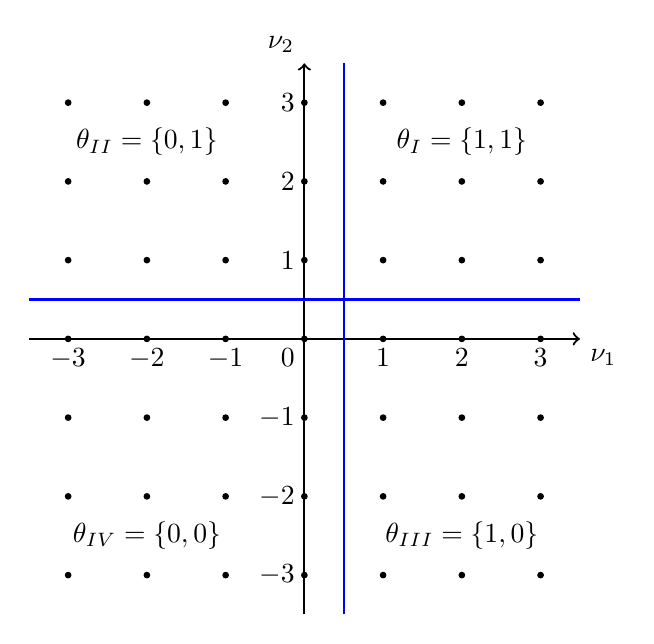
\begin{tikzpicture}
        %axes
        \draw[thick,->] (-3.5,0) -- (3.5,0) node[anchor=north west] {$\nu_1$};
        \draw[thick,->] (0,-3.5) -- (0,3.5) node[anchor=south east] {$\nu_2$};
        %dots and axes labels
        \draw[fill] (0,0) circle (1pt) node[anchor=north east] {$0$};
        \foreach \i in {-3,-2,-1,1,2,3}
            {
            \draw[fill] (0,\i ) circle (1pt) node[anchor=east] {$\i$};
            \draw[fill] (\i,0) circle (1pt) node[anchor=north] {$\i$};
            \foreach \j in {-3,-2,-1,1,2,3}
                \draw[fill] (\j, \i) circle (1pt);
            }
        %lines separating sectors
        \draw[thick, blue] (0.5, -3.5) -- (0.5, 3.5);
        \draw[thick, blue] (-3.5, 0.5) -- (3.5, 0.5);

        \node at (2, 2.5) {$\bm{\theta_I} = \{1, 1\}$};
        \node at (-2, 2.5) {$\bm{\theta_{II}} = \{0, 1\}$};
        \node at (2, -2.5) {$\bm{\theta_{III}} = \{1, 0\}$};
        \node at (-2, -2.5) {$\bm{\theta_{IV}} = \{0, 0\}$};

        \clip (-3.3,-3.3) rectangle (0.3, 0.3);
        \foreach \i in {-12,...,0}
            \draw[dashed, red, samples=100] plot function{-x+(0.3+0.5*\i)} node[right] {};
    \end{tikzpicture}
    \caption{Each point $(\nu_1, \nu_2)$ in the lattice $\mathbb{Z}^2$ corresponds to the $d$-dimensional Feynman integral $I(\nu_1, \nu_2)$. The lattice is divided into sectors as defined through Eq.~\ref{eq:sectors}. They are ordered as $\bm{\theta}_{I}>\bm{\theta}_{II},\,\bm{\theta}_{III}>\bm{\theta}_{IV}$. In particular, sector $\bm{\theta}_{IV}$ is trivially 0.} 
    \label{fig:IBPsectors}
    \end{subfigure}
    \hfill
    \hspace*{1em}\raisebox{0.9cm}{ % needed to align the diagrams
    \begin{subfigure}[b]{0.45\textwidth}
    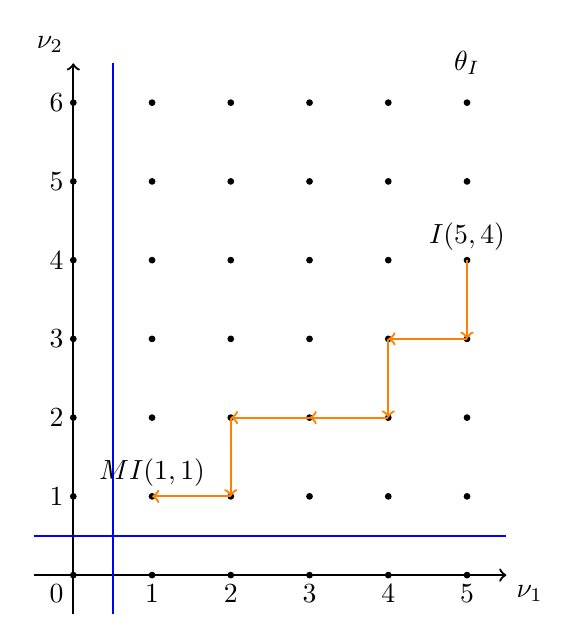
\begin{tikzpicture}
      %axes
        \draw[thick,->] (-0.5,0) -- (5.5,0) node[anchor=north west] {$\nu_1$};
        \draw[thick,->] (0,-0.5) -- (0,6.5) node[anchor=south east] {$\nu_2$};

        %dots and axes labels
        \draw[fill] (0,0) circle (1pt) node[anchor=north east] {$0$};
        \draw[fill] (0,6) circle (1pt) node[anchor=east] {$6$};
        \foreach \i in {1,...,5}
            {
            \draw[fill] (\i,0) circle (1pt) node[anchor=north] {$\i$};
            \draw[fill] (0,\i ) circle (1pt) node[anchor=east] {$\i$};
            \foreach \j in {1,...,6}
                {
                \draw[fill] (\i, \j) circle (1pt);
                }
            }

        %lines separating sectors
        \draw[thick, blue] (0.5, -0.5) -- (0.5, 6.5);
        \draw[thick, blue] (-0.5, 0.5) -- (5.5, 0.5);

        \draw[orange, thick, ->] (5, 4) edge (5,3) (5, 3) edge (4,3) (4,3) edge (4,2) (4,2) edge (3,2) (3,2) edge (2,2) (2,2) edge (2,1) (2, 1) -- (1,1);
        
        \node at (5, 6.5) {$\bm{\theta_I}$};
        \node at (1, 1) [anchor=south] {$\text{MI}(1, 1)$};
        \node at (5, 4) [anchor=south] {$I(5, 4)$};
    \end{tikzpicture}
    \caption{A hypothetical reduction pathway within the top sector $\bm{\theta}_I$. An integral $I(5, 4)$ is reduced to the master integral $\text{MI}(1,1)$ through a series of IBP relations lowering the denominator exponents.} \label{fig:IBPreduction}
    \end{subfigure}
    }
    \caption{A lattice of points visualising the integrals and sectors used in the IBP reduction ($N=2$).}
    \label{fig:IBPschematic}
\end{figure}
\begin{figure}
    \centering
        \begin{tikzpicture}
        	\begin{feynman}
        		\vertex (v1);
          
        		\vertex[right = of v1] (v2);			
        		\vertex[below = of v2] (v3);			
        		\vertex[left = of v3] (v4);			
          
        		\vertex[above left = 0.7cm of v1] (i1) {$p_1$};
        		\vertex[above right =  0.7cm of v2] (i2) {$p_2$};
        		\vertex[below right =  0.7cm of v3] (i3) {$p_3$};
        		\vertex[below left =  0.7cm of v4] (i4) {$p_4$};

                \node (dot) at ($(v2)!0.5!(v3)$);
                \draw[fill] (dot) circle (2pt);
          
        		\diagram*{
                    (v1) -- (v2) -- (v3) -- (v4) -- [momentum=$k_1$] (v1),
                    (i1) -- (v1),
                    (i2) -- (v2),
                    (i3) -- (v3),
                    (i4) -- (v4),
                    };
        	\end{feynman}
        \end{tikzpicture}
    \caption{One-loop box Feynman diagram $I_\text{box}(1,1,2,1)$ with a `dotted' propagator. The corresponding denominators are: $\{k_1^2, (k_1-p_1)^2, \left((k_1-p_1-p_2)^2\right)^2, (k_1+p_4)^2\}$\,.} \label{fig:1Lboxdot}
\end{figure}
It is now possible to order (albeit not uniquely) the sectors $\bm{\theta}$ with respect to each other, as well as the integrals $I_T(\bm{\nu})$ within each sector. It is natural to think of sectors with fewer unique denominators as simpler. Thus, $\sum_{i=1}^N \theta_i$ defines an ordering between the sectors. In the $N=2$ example, we say that the sector $\{1, 1\}$ is higher than its subsectors $\{1, 0\}$ and $\{0, 1\}$, which are both higher than their subsector $\{0, 0\}$ (which vanishes anyway). However, sectors $\{1, 0\}$ and $\{0, 1\}$ are equal. Within such equal sectors, we can define further criteria, for example based on the total power of the denominators, followed by the total power of the ISPs, etc. With the help of an arbitrary ordering, we can replace higher $I_T(\bm{\nu})$ by lower ones through the IBP reduction procedure, as visualised in Fig.~\ref{fig:IBPreduction}. It should not be surprising that the set of MIs remaining after this reduction depends on the ordering. We remark that, depending on our needs, it is possible to choose an ordering that leads to an ISP-free basis or conversely a dot-free basis, i.e without propagators raised to powers $\ge 2$ (see Fig.~\ref{fig:1Lboxdot}).

Overall, IBP relations allow us to express each helicity amplitude of Eq.~\ref{eq:ampreducedschematic} in terms of a much smaller number of integrals:
\begin{equation} \label{eq:ampafterIBP}
    	A_n^{(L)} \left(1^{h_1}, 2^{h_2}, \ldots, n^{h_n} \right) =  
     \sum_{i=1}^{|\text{MI}|} g_i(p, \eps) \times \text{MI}_i(p,\eps)\,,
\end{equation}
where $|\text{MI}|$ denotes the total number of linearly independent MIs in all the families. Once again, the coefficients are functions of external kinematics, as well as the dimensional regulator $\eps$. We emphasise that the step of IBP reducing the integrals involved in the amplitude can also be implemented over finite fields. In particular, the IBP system generated within the Laporta algorithm can be solved using \texttt{FiniteFlow}'s linear solver (for details, see Section~5 of~\cite{Peraro:2019svx}). This is an important simplification, since analytic IBP reduction often proves to be the bottleneck of the whole computation.

Moreover, in many applications, we will be dealing with multiple permutations of the maximal topologies appearing in Eq.~\ref{eq:ampreducedschematic}. In such cases, it is advantageous to implement an optimised strategy for obtaining the IBP solution in the permuted families, which is particularly powerful when used in conjunction with finite field techniques. It allows us to reduce the time and computational cost of the IBP reduction. We invite the reader to familiarise themselves with Appendix~\ref{app:altIBPs}, where we present this strategy in detail. We will exploit it when computing the QED amplitudes of Chapter~\ref{sec:QEDpaper}.

\section{Differential equations} \label{sec:DEs}
Differential equations (DEs) satisfied by Feynman integrals were studied even before the invention of the IBP reduction technique (see, for example, Refs.~\cite{Barucchi:1973zm, Golubeva:1976}). However, it was these two concepts combined together that led to the development of a powerful method for evaluating the MIs \cite{Kotikov:1990kg, Kotikov:1991314, Bern:1993kr, Remiddi:1997ny, Gehrmann:1999as}. The idea is as follows. If we differentiate an integral $I_T(\bm{\nu})$ with respect to the Mandelstam invariants, $s_{ij}$, or internal masses, $m_i^2$, we will obtain a linear combination of integrals within the same family $T$, but with different exponents $\bm{\nu}'$. These new integrals $I_T(\bm{\nu}')$ can then be IBP reduced onto the MIs of family $T$. Thus, if we apply the differentiation to the MI basis itself, we will obtain a set of first-order partial DEs (one for each kinematic variable). It is convenient to group the MIs as a vector $\vv{\text{MI}}$. We then have:
\begin{equation} \label{eq:DEspartial}
    \frac{\partial \vv{\text{MI}}}{\partial \lambda} = A_{\lambda}(\Lambda, \eps) \vv{\text{MI}}\,,
\end{equation}
where $\lambda \in \Lambda \equiv \{s_{ij}, m_i^2\}$ are the independent kinematic variables and $A_\lambda$ is a $\left(|\text{MI}| \times |\text{MI}|\right)$ matrix. Its entries are rational functions of $\Lambda$ and $\eps$, which is due to the nature of IBP relations. It is also common to work with the total differential rather than partial derivatives:
\begin{equation}
    \dd \vv{\text{MI}} = \sum_{\lambda} \left(\frac{\partial \vv{\text{MI}}}{\partial \lambda} \right) \dd \lambda\,,
\end{equation}
as well as to define:
\begin{equation}
    \dd A = \sum_\lambda A_\lambda \dd\lambda\,.
\end{equation}
Then, the system of DEs can be written as:
\begin{equation} \label{eq:DEsoneform}
    \dd \vv{\text{MI}} = \dd A(\Lambda, \eps) \,\vv{\text{MI}}\,.
\end{equation}
Naturally, to solve this equation, we also need to provide boundary values. Sometimes, it can be convenient to use the values of MIs at a special kinematic point, for example where one of the variables in $\Lambda_i$ vanishes or is equal to another kinematic variable. There, the MIs may become easier to evaluate. 
\subsection{The $\eps$-form} \label{sec:canonicalform}
In general, solving the DEs satisfied by MIs is hard. Note however, that typically we are interested in only the first few coefficients of the Laurent expansion of Eq.~\ref{eq:DEsoneform} around $\eps=0$. Consider a change of basis:
\begin{equation} \label{eq:basistransformation}
    \vv{\text{MI}} \rightarrow \vv{\text{MI}}^\prime = B\,\vv{\text{MI}}\,,
\end{equation}
where $B$ is an arbitrary matrix that can depend on $\Lambda$ and $\eps$. Under this transformation, the partial DEs become:
\begin{equation}
    \frac{\partial \vv{\text{MI}}^\prime}{\partial \lambda} = \left( \frac{\partial B}{\partial \lambda}B^{-1} + B A_{\lambda} B^{-1} \right) \vv{\text{MI}}^\prime\,.
\end{equation}
A key conjecture due to Ref.~\cite{Henn:2013pwa} is that it is always possible to choose $B$ such that:
\begin{equation}
    \left( \frac{\partial B}{\partial \lambda}B^{-1} + B A_{\lambda}(\Lambda, \eps) B^{-1} \right) = \eps \, \tilde{A}_{\lambda}(\Lambda)\,.
\end{equation}
That is, with an appropriate transformation, the $\eps$ dependence factorises out of the matrices, which now contain only kinematic dependence. Note, however, that they might contain algebraic (i.e. non-rational) factors such as square roots. Overall, Eq.~\ref{eq:DEspartial} becomes:
\begin{equation} \label{eq:canonicalDEspartial}
    \frac{\partial \vv{\text{MI}}^\prime}{\partial \lambda} = \eps \, \tilde{A}_{\lambda}(\Lambda) \, \vv{\text{MI}}^\prime\,, 
\end{equation}
while Eq.~\ref{eq:DEsoneform}:
\begin{equation} \label{eq:canonicalDEsoneform}
    \dd \vv{\text{MI}}^\prime = \eps \, \dd \tilde{A}(\Lambda) \,\vv{\text{MI}}^\prime\,.
\end{equation}
This is known as DEs in the `$\eps$-form' \footnote{Several packages exist for transforming the DEs into the $\eps$-form. See \texttt{Fuchsia}~\cite{Gituliar:2017vzm}, \texttt{Libra}~\cite{Lee:2020zfb}, \texttt{INITIAL}~\cite{Dlapa:2020cwj} and \texttt{CANONICA}~\cite{Meyer:2018feh}. See also \cite{Dlapa:2022nct} for a comprehensive review of different techniques.}. We will henceforth drop the superscript $^\prime$ on the vector of MIs as we will always be dealing with DEs in this form. In particular, Eq.~\ref{eq:canonicalDEsoneform} admits a solution in terms of the path-ordered exponential:
\begin{equation} \label{eq:pathexponential}
    \vv{\text{MI}}(\Lambda, \eps) = \mathbb{P} \exp \left(\eps\int_\gamma \dd \tilde{A} \right) \vv{\text{MI}}(\Lambda_0, \eps )\,,
\end{equation}
where $\gamma\,:\,[0, 1] \rightarrow \mathbb{C}^{|\Lambda|}$ is a path in the space of the kinematic invariants, with $\Lambda = \gamma(1)$ and $\Lambda_0 = \gamma(0)$. We remark that the integral is independent of the path taken as long as the two paths can be continuously deformed into each other without crossing the poles of the DEs. Because the solution is expressed through a series expansion of the matrix exponential, it is easy to see that the MIs are obtained as iterated integrals of $\tilde{A}$. Given the Laurent expansion of the MI vector:
\begin{equation} \label{eq:MIlaurentexp}
    \vv{\text{MI}}(\Lambda, \eps) = \sum_{k=0}^\infty \eps^k\,\vv{\text{MI}}^{(k)}(\Lambda) \,,
\end{equation}
we can insert it into Eq.~\ref{eq:pathexponential} and series expand both its sides in $\eps$. Then, the order-by-order DE solution becomes:
\begin{equation} \label{eq:DEssolution}
    \vv{\text{MI}}^{(k)}(\Lambda) = \sum_{j=0}^k \int_\gamma \underbrace{\dd \tilde{A} \cdot \ldots \cdot \dd \tilde{A}}_{j\text{ times}} \, \cdot \, \vv{\text{MI}}^{(k-j)}(\Lambda_0)\,.
\end{equation}
The integrals:
\begin{equation} \label{eq:CIIsdef}
    \int_\gamma \dd \Omega_1 \cdot \ldots \cdot \dd \Omega_j = \int_{0}^1 \frac{\partial \Omega_j(\gamma(t_j))}{\partial t_j} \dd t_j \int_{0}^{t_j} \frac{\partial \Omega_{j-1}(\gamma(t_{j-1}))}{\partial t_{j-1}} \dd t_{j-1} \cdots \int_{0}^{t_2} \frac{\partial \Omega_1(\gamma(t_1))}{\partial t_1} \dd t_1 \,,
\end{equation}
where $\dd \Omega_i$ are exact one-forms, are known as Chen's iterated integrals (CIIs)~\cite{Chen:1977oja}. We refer the reader to Refs.~\cite{Brown:2013qva, Abreu:2022mfk} for a thorough discussion of their properties. The empty CII, i.e. Eq.~\ref{eq:CIIsdef} for $j=0$, is defined as 1. Finally, we point out that we can assume that the Laurent expansion in Eq.~\ref{eq:MIlaurentexp} starts from $\eps=0$, because the DEs are insensitive to a rescaling of the integrals by a factor which does not depend on the kinematics. Thus, the MIs can be normalised to be finite, which moves any potential singularities at $\eps=0$ into their coefficients. 
\subsection{The $\dd \log$ form and Goncharov Polylogarithms} \label{sec:DEdlogform}
Overall, we see that the MIs at $\order{\eps^k}$ are given by sums of up to $k$-fold integrals. The integration kernels are determined by the structure of the matrices $\tilde{A}$, which deserves further discussion. Let us consider the singularities of the DEs. It can be shown, for example by studying the Feynman parameter representation, that Feynman integrals cannot contain so-called essential singularities, e.g. singularities of the form $\mathrm{e}^{1/\lambda} = 1+ 1/\lambda + 1/(2!\lambda^2)+\ldots\,$ at $\lambda=0$. In particular, for each singularity $\lambda^\ast$, the leading behaviour of Feynman integrals is $\sim (\lambda- \lambda^\ast)^\alpha$ for some power $\alpha$. This strongly constrains the form that the corresponding DE matrices can take\cite{Henn:2014qga}. Specifically, we expect them to have simple poles of the form $\sim \alpha/(\lambda-\lambda^\ast)$ for each $\lambda^\ast$. The $\eps$-form DEs of Eqs.~\ref{eq:canonicalDEspartial} and \ref{eq:canonicalDEsoneform} satisfying this additional `fuchsian' property are referred to as `canonical DEs' \footnote{In practice, when constructing canonical DEs, we might encounter spurious double poles or higher. For one-variable problems, they can be algorithmically removed by a suitable basis change which leaves the DEs with only simple poles in this variable. However, for multi-variable problems, it is a conjecture that this can be achieved simultaneously for all variables (see Ref.~\cite{Dlapa:2022nct} for details).}.

Furthermore, in many cases of practical interest, it is possible to construct MI bases which result in DEs in the so-called `$\dd \log$ form':
\begin{equation} \label{eq:dlogform}
    \dd\tilde{A} = \sum_{i=1}^{|\bm{w}|} a_i \times \dd \log w_i\,.
\end{equation}
Here, $w_i$ are known as `letters' (note that sometimes the differentials $\dd \log w_i$ are referred to as letters instead), while their collection $\bm{w} = \{w_1, w_2, \ldots\}$ is the `alphabet'. The matrices $a_i$ contain rational numbers only, free of any kinematic and $\eps$ dependence. The letters play a central role in the analysis of DEs in the $\dd \log$ form, since they control their singularities and determine which class of special functions the MIs are written in terms of. As mentioned before, in general the kinematic dependence of $\tilde{A}$ might no longer be rational, as the transformation Eq.~\ref{eq:basistransformation} needed to bring DEs into canonical form might introduce non-rational functions into the definitions of the corresponding canonical MIs. In this case, the letters $w_i$ are algebraic functions of $\Lambda$. However, if the form of Eq.~\ref{eq:dlogform} can be reached using rational transformations only, the letters are also rational functions. Then, it is particularly easy to write down the order-by-order solution in Eq.~\ref{eq:DEssolution}, as the iterated integrals become the well-known Goncharov Polylogarithms (GPLs)\footnote{Also known as Multiple Polylogarithms (MPLs).}\cite{2001math......3059G, 2011arXiv1105.2076G, Vollinga:2004sn}:
\begin{equation} \label{eq:GPLs}
    G_n(a_1, a_2, \ldots, a_n; x) = \int_0^x \frac{\dd t}{t-a_1} G_{n-1}(a_2, \ldots, a_n; t)\,,
\end{equation}
with the `empty' GPL:
\begin{equation}
    G_0(; x) = 
    \begin{cases}
        0 & \text{if } x = 0\,, \\
        1 & \text{if } x \neq 0\,. 
    \end{cases}
\end{equation}
Here, despite the somewhat suggestive notation, the indices $a_i$ do not have to be numbers and are considered fully-fledged arguments of $G_n$, alongside $x$. The length of the vector $\vec{a} = (a_1, \ldots a_n)$, i.e. $|\vec{a}|=n$, is called the weight (or depth) of $G_n$. The GPLs are related to the usual logarithms through:
\begin{subequations}
   \begin{align}
    G_n(a, a, \ldots, a; x) &= 
        \frac{1}{n!}\log^n\left(1-\frac{x}{a}\right) \quad \text{if } a \neq 0\,, \label{eq:GPLtolognonzero} \\ 
    G_n(0, 0, \ldots, 0; x) &= 
        \frac{1}{n!}\log^n x \,. \label{eq:GPLtologzero}
   \end{align} 
\end{subequations}
Aside from this special case of GPLs, the complexity of the integration kernels can be estimated by studying the maximal cuts of the relevant Feynman integrals~\cite{Tancredi:2017onthemaxcut, Abreu:2020jxa, abreu2021twoloop}. More generally, the letters might not be rational, or the kernels overall might not be of the $\dd \log$ form. Then, more complicated functions appear in the solution of the DEs.  For example, the presence of internal masses in the Feynman diagrams often leads to Elliptic Multiple Polylogarithms (eMPLs). We refer the reader to Refs.~\cite{Broedel:2017kkb, Broedel:2017siw, Adams:2017ejb, Broedel:2018qkq, Adams:2018yfj, Walden:2020odh} for a discussion of eMPLs and also to Refs.~\cite{Bonciani:2016qxi, Bonciani:2019jyb, Frellesvig:2019byn} for a closer look at their application to Higgs+jet production with quark mass dependence.

\subsection{Uniform transcendentality} \label{sec:UT}
When talking about the canonical DEs, it is also useful to introduce the idea of `transcendentality'. For an iterated integral $f$, its transcendental weight $\mathcal{T}$ is simply the number of iterated integrations needed to define $f$\cite{Henn:2013pwa}. For example, $\mathcal{T}(\log x) = 1$, while $\mathcal{T}(G_n(a_1, \ldots, a_n;\, x)) = n$. From this definition, it follows that $\mathcal{T}(f_1 f_2) = \mathcal{T}(f_1) + \mathcal{T}(f_2)$, but note that $\mathcal{T}(f_1 + f_2)$ cannot be defined unless $\mathcal{T}(f_1) = \mathcal{T}(f_2)$. Furthermore, algebraic functions and constants have weight 0. Transcendental constants which can be obtained as values of transcendental functions at algebraic arguments have the corresponding weight, e.g. $\mathcal{T}(\pi) = 1$, since $\log (-1) = \pm \i \pi$ and $\mathcal{T}(\mathrm{i}) = \mathcal{T}(-1) = 0$, while $\mathcal{T}(\zeta(n)) = n$, since $\zeta(n) = \text{Li}_n(1)$ (for $n>1$)\footnote{Here, $\text{Li}_n(z)$ are the classical polylogarithms, which we discuss in Appendix~\ref{app:symbols}.}. It is also convenient to assign $\mathcal{T}(\eps)=-1$. With this choice, it is clear that every term in the solution of Eq.~\ref{eq:pathexponential} has the same transcendental weight. This property is referred to as `uniform transcendentality' (UT). A simple example of a UT function is $f(x) = 1 + \eps (\log x + \pi) + \eps^2 (\log^2 x + G_2(1, 1;\, x))$, with $\mathcal{T}(f) = 0$. Additionally, UT functions satisfying a more stringent condition:
\begin{equation} \label{eq:purecondition}
    \mathcal{T}(\dd f) = \mathcal{T}(f) - 1\,,
\end{equation}
are known as `pure' function. In practice, this means that a pure function cannot contain algebraic factors that are not constant --- while they do not affect the transcendental weight of a function, they affect the DE it satisfies\footnote{Note that in literature, the term `UT' is often implicitly taken to mean `pure'.}. As an example, the function $f(x) = \log(x)/x + \ii \pi$ is UT, but not pure. It immediately follows that the iterated integral solution to the $\eps$-form DEs is built out of pure functions. The reverse is also true: given a pure basis of MIs, the DEs they satisfy will be in the $\eps$-form. In practice, when constructing a MI basis, we can verify the validity of the $\eps$-free matrices $\tilde{A}_\lambda$ in Eq.~\ref{eq:canonicalDEspartial} by checking the following conditions:
\begin{subequations}
\begin{align}
    [ \tilde{A}_{\lambda_i}, \tilde{A}_{\lambda_j}] &= 0\,, \\
    \partial_{\lambda_i} \tilde{A}_{\lambda_j} - \partial_{\lambda_j} \tilde{A}_{\lambda_i} &= 0\,, \\
    %\sum_{\lambda \in \Lambda} \lambda \, \eps \, \tilde{A}_\lambda \cdot \vv{\text{MI}} &= \eps \, \text{diag}([\text{MI}_1], [\text{MI}_2], \ldots) \cdot \vv{\text{MI}} \,,
    \sum_{\lambda \in \Lambda} \lambda \, \tilde{A}_\lambda &= \text{diag}([\text{MI}_1], [\text{MI}_2], \ldots)\,,
\end{align}
\end{subequations}
where the sum runs over all kinematic scales and $[\text{MI}_i]$ is the mass dimension of MI$_i$. The first two equations follow from integrability conditions, while the last one follows from Euler's homogeneous function theorem. Finally, we point out an interesting observation on the nature of dimensionally regulated amplitudes (see e.g. Ref.~\cite{Duhr:2014woa}). For a Laurent expanded $L$-loop amplitude in $d = 4- 2\eps$, it is conjectured that the $\order{\eps^k}$ term contains functions of transcendental weight up to $2L+k$. For example, to calculate a two-loop amplitude up to $\order{\eps^0}$, we need to supply the MI expansions up to weight 4. It is expected that in $\mathcal{N}=4$ Super Yang-Mills theory, this bound is saturated, i.e. functions of weight \textit{exactly} $2L+k$ are required.
\begin{table}[t]
	\begin{center}
		\begin{tabular}{|c|c|c|c|}
            \hline
            External masses & Type & Topology & Publications \\
			\hline
            \multirow{2}{0cm}{0} & planar & penta-box & \cite{Gehrmann:2015bfy,Papadopoulos:2015jft, Gehrmann:2018yef, Abreu:2018aqd, Chicherin:2020oor} \\
            \cline{2-4}
            & \multirow{2}{2cm}{non-planar} & hexa-box & \cite{Chicherin:2018mue, Chicherin:2017dob, Chicherin:2018ubl, Chicherin:2018wes, Abreu:2018rcw, Chicherin:2020oor, Abreu:2018aqd} \\
            & & double-pentagon & \cite{Chicherin:2018old, Abreu:2018aqd, Chicherin:2020oor} \\
            \hline
            \multirow{2}{0cm}{1} & planar & penta-box & \cite{Papadopoulos:2015jft, Abreu:2020jxa, Chicherin:2021dyp, Canko:2020ylt} \\
            \cline{2-4}
            & \multirow{2}{2cm}{non-planar} & hexa-box & \cite{abreu2021twoloop, Kardos:2022tpo, Papadopoulos:2019iam, Chicherin:2021dyp} \\
            & & double-pentagon & \cite{Abreu:2023rco} \\
            \hline
		\end{tabular}
\end{center}
\caption{Selected works relevant to the computation of two-loop, five-point pure MI bases. All propagators are massless.}
\label{tab:MIs}
\end{table}

Overall, pure integrals have played a central role in the derivation and evaluation of MI bases relevant to this thesis, that is bases for processes with a high number of kinematic scales. For future convenience, in Table~\ref{tab:MIs} we collect (without claiming to be exhaustive) the publications dealing with the MI bases for two-loop, five-point processes with up to one external mass and massless propagators. Finally, before moving on, we invite the reader to familiarise themselves with the content of Appendix~\ref{app:symbols}, which introduces the notion of a `symbol'. It is yet another concept related to the study of DEs satisfied by Feynman integrals and we aim to show its usefulness through several illustrative examples.

\section{Evaluating master integrals}
After a rather lengthy excursion into the world of IBPs and DEs, let us remind ourselves where we currently stand in the workflow for computing amplitudes presented in Fig.~\ref{fig:outline}. Having written down the helicity-dependent numerators of each colour-ordered amplitude, we were faced with the task of integrating an enormous number of tensor integrals that belong to many integral topologies. Then, in Section~\ref{sec:reduction}, we mapped all these integrals onto integrals within significantly fewer \textit{maximal} topologies. We then built a system of IBP relations for each of these maximal topologies and reduced the integrals further onto a manageable set of MIs. In principle, we can now end the amplitude computation. Our result is written in terms of rational coefficients of external kinematics and $\eps$, which are trivial to evaluate over the full phase space, while the MIs that these coefficients multiply are in general functions that are extremely hard to compute analytically and that exhibit a complicated branch cut structure. As we will see in the next section, there are good reasons why we typically extend our workflow and express the MIs in terms of appropriately chosen special functions. However, it is entirely possible to work with the amplitude at the level of MIs. Indeed, in some cases we have no other choice, since the expansion of the relevant MIs into special functions may not be known. Having phenomenological applications in mind, we list below a few methods which allow us to evaluate these MIs numerically at chosen kinematic points. In fact, we will use the last two in subsequent chapters.
\begin{itemize}
    \item \textbf{Sector decomposition}: This method relies on the parametrisation of integrals in terms of the Feynman parameters and the $\mathcal{U}$ and $\mathcal{F}$ Symanzik polynomials. The integration phase space of the parameters is split into sectors and subsectors based on a relative ordering between the parameters. This allows us to resolve the singularities present in the integrals and place them in simple functions that can be integrated analytically. What remains to be computed are the coefficients of the $\eps$ poles. They receive contributions from finite integrals only and are computed numerically~\cite{Binoth:2000ps, Binoth:2003ak}. There exist several public codes implementing this algorithm~\cite{Bogner:2007cr, Smirnov:2015mct, Borowka:2015mxa, Heinrich:2023til}.
    \item \textbf{Expansion by regions}: In this method, the integration domain of the loop momenta is divided into appropriate regions where a certain kinematic quantity is small, e.g. $m_i^2/p_j^2 \ll 1$. For each such limit, the integrand is expanded in the corresponding small parameter and the expansion is truncated at a certain order, resulting in a simpler approximation. The expanded integrands are then integrated over the \textit{full} space of loop momenta. With certain conditions ~\cite{Jantzen:2011nz}, the original integral can be recovered by summing the individual contributions from the various regions~\cite{Beneke:1997zp, Smirnov:1998vk, Smirnov:1999bza, Pak:2010pt, Ananthanarayan:2018tog}. For numerical implementation, see Refs.~\cite{Ananthanarayan:2020ptw, Jantzen:2012mw, Smirnov:2015mct, Heinrich:2021dbf}. 
    \item \textbf{Generalised series expansion}: For integrals satisfying a set of DEs, it is possible to integrate these DEs along a one-dimensional line segment\footnote{We stress that this method is applicable not only to MIs, but to any set of functions satisfying DEs. We will explore this further in Chapter~\ref{sec:Hbb}.}. If we know the value of the integrals at one point in the kinematic phase space (i.e. the boundary condition of the DEs) and want to know their value at another point, we construct a path $\gamma(t)$ between them and solve the DEs along it. Thus, the task is reduced to a one-dimensional problem in the parameter $t$ of the path, with all the kinematic invariants set to numerical values. The solution is then obtained by using an ansatz in the form of a series expansion. 

    Naturally, each such series has a certain radius of convergence within which it is valid. Typically, it is the distance from the centre point of the expansion to the nearest singularity. Thus, in order to obtain the full solution across the entire length of $\gamma(t)$, we split the path into multiple segments and solve the DEs on them one by one. The value of the solution from the previous segment can then serve as a boundary condition for solving the DEs in the subsequent segment~\cite{Moriello:2019yhu, Bonciani:2019jyb, Frellesvig:2019byn}. We provide a more intuitive, graphical representation of this idea in Fig.~\ref{fig:seriesexp}. Recently, public implementations of this method have been presented in Refs.~\cite{Hidding:2020ytt, Armadillo:2022ugh}.
    \item \textbf{Auxiliary mass flow}: This method relies on constructing the DEs not with respect to the traditional kinematic invariants, but an auxiliary mass parameter $\eta$. The original integrals can then be recovered by solving the $\eta$-DEs with $\eta = \infty$ as the boundary condition and letting $\eta$ `flow' from $\infty$ to $\ii \varepsilon^-$. Crucially, the integrals involved in the boundary condition are simpler than the ones we are aiming for. If these prove still too hard to compute, we can iterate the procedure: set up new $\eta^\prime$-DEs for these integrals, obtain the new boundary condition in terms of even simpler integrals, and so on. Eventually, the boundary terms can be expressed in terms of scaleless integrals (which vanish in DR) or single-scale vacuum integrals (which are very simple)~\cite{Liu:2017jxz, Liu:2021wks}. A public implementation of this method has been made available in Ref.~\cite{Liu:2022chg}.
\end{itemize}
\begin{figure}
    \centering
    \begin{tikzpicture}
		\node (start) at (0,0) {};
		\node (startcaption) at ([yshift=-2pt]start.south) {$s_0$};
		\node (i1) [right of=start, xshift=1em, yshift=0.5em] {};
		\node (i2) [right of=i1, xshift=0.9em, yshift=-1.8em] {};
		\node (finish) [right of=i2, xshift=1em, yshift=1em] {};
		\node (finishcaption) at ([yshift=-2pt]finish.south) {$s$};
        \node (label1) [right of=i1, xshift=-0.6cm, yshift=-0.2cm] {};
        \node (label2) [above right= 1cm of label1] {$\gamma(t)$};
		
		\foreach \i in {start,i1,i2,finish}{
			\filldraw[red] (\i.center) circle (0.1em);
			\draw[red,dashed] (\i.center) circle (2.1em);
		}
		\draw (start.center) to [out=70,in=250] (i1.center) to [out=70,in=180] (i2.center) to [out=0,in=90] (finish.center);
        \draw [{Stealth[scale=1.5]}-] (label1) -- (label2);
	\end{tikzpicture}
    \caption{A pictorial representation of the generalised series expansion method. We connect the kinematic point $s_0 = \gamma(0)$, at which the solution to the DEs is known, to the target point $s = \gamma(1)$ with a one-parameter path $\gamma(t)$. The path is split into segments as necessitated by singularities. On each segment, we express the solution to the DEs in the form of a series expansion which has a certain radius of convergence (marked by dashed circles). Stitching together the solutions from individual segments allows us to transport the solution from $s_0$ to $s$.}
    \label{fig:seriesexp}
\end{figure}
\section{Special functions and finite remainders} \label{sec:specialfunctions}
The techniques listed above are very flexible and general. They are not in principle limited to a particular loop order or kinematic configuration, although naturally we expect a drop in performance as we move to more complicated integrals. We also point out that they do not require the MIs to be pure. Overall, following these methods, we are able to evaluate a wide class of integrals. However, the evaluation time is not fast enough for the phenomenological applications of the amplitudes presented in our work. For this reason, we usually resort to a more fine-tuned approach, which we describe below. 

After reducing the amplitude onto a small set of MIs, we make use of the available results for these MIs and expand them onto a basis of special functions, which we will denote as $\{f_i(p)\}$ for now, with $p$ indicating the collective dependence on external momenta. These functions could involve, e.g. GPLs, eMPLs or other case-specific functions better suited to a particular computation. More details on this topic will be presented in Sections~\ref{Hbbsec:Hbasis}, \ref{wyjsec:Permutations} and \ref{secQED:spec-fns}. The expansion of MIs onto $\{f_i(p)\}$ can be easily implemented over the finite fields as a multiplication of the MI coefficients $g_i(p, \eps)$ in Eq.~\ref{eq:ampafterIBP} by a matrix encoding these MIs in terms of the special functions. Schematically, we are left with:
\begin{equation} \label{eq:ampexpandedspfuncs}
    A_n^{(L)} \left(1^{h_1}, 2^{h_2}, \ldots, n^{h_n} \right) = \sum_i q_i(p, \eps) \times \text{mon}_i \big(\{f_i(p)\}\big)\,,
\end{equation}
where mon$_i$ denote monomials formed from the special functions.

In contrast with the methods described in the previous section, special functions are not a solution that generalises easily, in the sense that their construction is difficult and has to be done case by case. Nonetheless, expanding the amplitude onto a basis of special functions has several advantages. First and foremost, all cancellations and simplifications are manifest, leading to a unique representation of the amplitude. This is an important improvement in the context of the finite field framework, as it means that we will not have to reconstruct additional, `unphysical' coefficients. It also unveils the analytic structure that is simply hidden within the MI representation. Furthermore, having a basis of special functions grants us a more efficient numerical evaluation of a minimal number of functions. Finally, it allows us to subtract from the amplitude its UV and IR poles and define the so-called `finite remainder':
\begin{equation} \label{eq:finremschematic}
    F^{(L)} = \lim_{\eps \to 0} \left( A^{(L)} - P^{(L)} A^{(0)} \right)\,,
\end{equation}
where the $L$-loop pole operator $P^{(L)}$ contains both UV and IR divergences. We stress that $P^{(L)}$ contains contributions from amplitudes at loop orders $l<L$. For a detailed discussion, we refer the reader to subsequent chapters and Appendix~\ref{app:polestructure}.

A few words on why we want to work with the finite remainder are in order. Since the UV poles of an amplitude are eliminated in renormalisation, while the IR poles are determined from lower-loop information~\cite{Catani:1998bh, Becher:2009cu, Becher:2009qa, Gardi:2009qi}, the genuinely new information we compute is contained solely in the non-singular terms. Moreover, the fact of being able to subtract these pre-determined poles from our result, such that we are left with a finite quantity in the limit $\eps \rightarrow 0$, is in itself already a strong check on the calculation. Finally, it has been observed that finite remainders often exhibit simpler analytic structure than the corresponding full amplitude, with certain special functions dropping out after subtracting the poles. Thus, it is the finite remainder, rather than the amplitude itself, that we take as the end point of our computational algorithm in Fig.~\ref{fig:outline}:
\begin{equation}
    F_n^{(L)} \left(1^{h_1}, 2^{h_2}, \ldots, n^{h_n} \right) = \sum_i r_i(p) \times \text{mon}_i \big(\{f_i(p)\}\big)\,.
\end{equation}
Let us make three remarks about the finite remainder. First, we emphasise that it is dependent on the renormalisation, regularisation and IR subtraction schemes. It is important to bear that in mind when cross-checking results or trying to restore the full amplitude from its remainder. Second, the pole subtraction in Eq.~\ref{eq:finremschematic} can be straightforwardly implemented over finite fields as a subtraction on the coefficients $q_i$ in Eq.~\ref{eq:ampexpandedspfuncs}. Third, due to the simplifications that occur during this subtraction, the reconstruction of the finite remainder coefficients $r_i$ is usually easier as compared to the reconstruction of $q_i$.

While the special functions $\{f_i\}$ that come from the MIs are complicated functions with singularities and branch cuts, the coefficients $r_i$ are rational functions that are computed and reconstructed from finite fields. We remind the reader that they will be usually expressed in terms of the MTs (see Section~\ref{sec:MTs}). In practical applications at the state of the art, the reconstruction processes can be enormously expensive even on modern CPU clusters. For this reason, we find it unavoidable to implement several tools which simplify the coefficients before we need to reconstruct them. They lower the polynomial degrees and will be covered in detail when discussing the reconstruction strategies in Sections~\ref{Hbbsec:reduction} and \ref{wyjsec:Reconstruction}.

We are now ready to take on the computation of scattering amplitudes at the cutting edge of current knowledge. In subsequent chapters, we will use the workflow developed here to tackle two-loop amplitudes for three processes directly relevant to modern particle physics phenomenology.
\end{document}